% Options for packages loaded elsewhere
\PassOptionsToPackage{unicode}{hyperref}
\PassOptionsToPackage{hyphens}{url}
\PassOptionsToPackage{dvipsnames,svgnames,x11names}{xcolor}
%
\documentclass[
  11pt,
]{article}

\usepackage{amsmath,amssymb}
\usepackage{lmodern}
\usepackage{iftex}
\ifPDFTeX
  \usepackage[T1]{fontenc}
  \usepackage[utf8]{inputenc}
  \usepackage{textcomp} % provide euro and other symbols
\else % if luatex or xetex
  \usepackage{unicode-math}
  \defaultfontfeatures{Scale=MatchLowercase}
  \defaultfontfeatures[\rmfamily]{Ligatures=TeX,Scale=1}
\fi
% Use upquote if available, for straight quotes in verbatim environments
\IfFileExists{upquote.sty}{\usepackage{upquote}}{}
\IfFileExists{microtype.sty}{% use microtype if available
  \usepackage[]{microtype}
  \UseMicrotypeSet[protrusion]{basicmath} % disable protrusion for tt fonts
}{}
\makeatletter
\@ifundefined{KOMAClassName}{% if non-KOMA class
  \IfFileExists{parskip.sty}{%
    \usepackage{parskip}
  }{% else
    \setlength{\parindent}{0pt}
    \setlength{\parskip}{6pt plus 2pt minus 1pt}}
}{% if KOMA class
  \KOMAoptions{parskip=half}}
\makeatother
\usepackage{xcolor}
\usepackage[top=30mm,left=20mm]{geometry}
\setlength{\emergencystretch}{3em} % prevent overfull lines
\setcounter{secnumdepth}{5}
% Make \paragraph and \subparagraph free-standing
\ifx\paragraph\undefined\else
  \let\oldparagraph\paragraph
  \renewcommand{\paragraph}[1]{\oldparagraph{#1}\mbox{}}
\fi
\ifx\subparagraph\undefined\else
  \let\oldsubparagraph\subparagraph
  \renewcommand{\subparagraph}[1]{\oldsubparagraph{#1}\mbox{}}
\fi


\providecommand{\tightlist}{%
  \setlength{\itemsep}{0pt}\setlength{\parskip}{0pt}}\usepackage{longtable,booktabs,array}
\usepackage{calc} % for calculating minipage widths
% Correct order of tables after \paragraph or \subparagraph
\usepackage{etoolbox}
\makeatletter
\patchcmd\longtable{\par}{\if@noskipsec\mbox{}\fi\par}{}{}
\makeatother
% Allow footnotes in longtable head/foot
\IfFileExists{footnotehyper.sty}{\usepackage{footnotehyper}}{\usepackage{footnote}}
\makesavenoteenv{longtable}
\usepackage{graphicx}
\makeatletter
\def\maxwidth{\ifdim\Gin@nat@width>\linewidth\linewidth\else\Gin@nat@width\fi}
\def\maxheight{\ifdim\Gin@nat@height>\textheight\textheight\else\Gin@nat@height\fi}
\makeatother
% Scale images if necessary, so that they will not overflow the page
% margins by default, and it is still possible to overwrite the defaults
% using explicit options in \includegraphics[width, height, ...]{}
\setkeys{Gin}{width=\maxwidth,height=\maxheight,keepaspectratio}
% Set default figure placement to htbp
\makeatletter
\def\fps@figure{htbp}
\makeatother
\newlength{\cslhangindent}
\setlength{\cslhangindent}{1.5em}
\newlength{\csllabelwidth}
\setlength{\csllabelwidth}{3em}
\newlength{\cslentryspacingunit} % times entry-spacing
\setlength{\cslentryspacingunit}{\parskip}
\newenvironment{CSLReferences}[2] % #1 hanging-ident, #2 entry spacing
 {% don't indent paragraphs
  \setlength{\parindent}{0pt}
  % turn on hanging indent if param 1 is 1
  \ifodd #1
  \let\oldpar\par
  \def\par{\hangindent=\cslhangindent\oldpar}
  \fi
  % set entry spacing
  \setlength{\parskip}{#2\cslentryspacingunit}
 }%
 {}
\usepackage{calc}
\newcommand{\CSLBlock}[1]{#1\hfill\break}
\newcommand{\CSLLeftMargin}[1]{\parbox[t]{\csllabelwidth}{#1}}
\newcommand{\CSLRightInline}[1]{\parbox[t]{\linewidth - \csllabelwidth}{#1}\break}
\newcommand{\CSLIndent}[1]{\hspace{\cslhangindent}#1}

%----------------------------------------------------
% 	CONFIGURATION OF PARAMETERS
%----------------------------------------------------

\let\paragraph\oldparagraph
\let\subparagraph\oldsubparagraph

\usepackage{titlesec}
\newcommand{\sectionbreak}{\clearpage}

% ----------------
%  FONTS AND TYPESETTING SETTINGS
% -----------------
%\usepackage[french]{babel}
%\usepackage[bitstream-charter]{mathdesign}

\usepackage{fontawesome5}
\usepackage{academicons}
\usepackage[notransparent]{svg}
\usepackage{tabu}
%\usepackage{coloremoji}
%\usepackage{emoji}
%\usepackage{longtable}

%\usepackage[tracking=smallcaps]{microtype}
%\usepackage[bitstream-charter]{mathdesign}

% ----------------
%  STYLES OF THE CHAPTER, SECTION
% -----------------
%Options: Sonny, Lenny, Glenn, Conny, Rejne, Bjarne, Bjornstrup
% \usepackage[Bjornstrup]{fncychap}
% \usepackage{marginnote}
% \renewcommand*{\marginfont}{\small\sffamily}
% \usepackage{wrapfig}



% -----------------
%  VARIOUS PACKAGES FROM ME
% -----------------
%\usepackage{minitoc}
%\usepackage{float} % Required for tables and figures in the multi-column environment - they need to be placed in specific locations with the [H] (e.g. \begin{table}[H])
%\usepackage[lofdepth,lotdepth]{subfig} 
%\usepackage{multirow} % Use multirows in the tables

%\usepackage {textcomp} % (Symbols Euros)
%\usepackage{nomencl} % nomenclature package
%\usepackage{soul}
%\renewcommand\thesection{\arabic{section}} %Redefinition of numeration of the document
%\usepackage{pdflscape} % hacer el documento lanscape en las hojas
%\usepackage{enumitem} % offers ready-made options for eliminating the space between items and paragraphs within the list (noitemsep) or all vertical spacing (nosep): 

%\usepackage{afterpage} % For make blank pages
\usepackage{pdfpages} % For insert the title page.




% -----------------
%  VARIOUS PACKAGES FROM UNIVERSITE DE LORRAINE
% -----------------
\usepackage{import}



% -----------------
%  DEFINITION OF COMMANDS BY ME
% -----------------
%\pagenumbering{Roman}


\newenvironment{cols}[1][]{}{}

\newenvironment{col}[1]{\begin{minipage}{#1}\ignorespaces}{%
\end{minipage}
\ifhmode\unskip\fi
\aftergroup\useignorespacesandallpars}

\def\useignorespacesandallpars#1\ignorespaces\fi{%
#1\fi\ignorespacesandallpars}

\makeatletter
\def\ignorespacesandallpars{%
  \@ifnextchar\par
    {\expandafter\ignorespacesandallpars\@gobble}%
    {}%
}
\makeatother


\usepackage{booktabs}
\usepackage{longtable}
\usepackage{array}
\usepackage{multirow}
\usepackage{wrapfig}
\usepackage{float}
\usepackage{colortbl}
\usepackage{pdflscape}
\usepackage{tabu}
\usepackage{threeparttable}
\usepackage{threeparttablex}
\usepackage[normalem]{ulem}
\usepackage{makecell}
\usepackage{xcolor}
\makeatletter
\@ifpackageloaded{tcolorbox}{}{\usepackage[many]{tcolorbox}}
\@ifpackageloaded{fontawesome5}{}{\usepackage{fontawesome5}}
\definecolor{quarto-callout-color}{HTML}{909090}
\definecolor{quarto-callout-note-color}{HTML}{0758E5}
\definecolor{quarto-callout-important-color}{HTML}{CC1914}
\definecolor{quarto-callout-warning-color}{HTML}{EB9113}
\definecolor{quarto-callout-tip-color}{HTML}{00A047}
\definecolor{quarto-callout-caution-color}{HTML}{FC5300}
\definecolor{quarto-callout-color-frame}{HTML}{acacac}
\definecolor{quarto-callout-note-color-frame}{HTML}{4582ec}
\definecolor{quarto-callout-important-color-frame}{HTML}{d9534f}
\definecolor{quarto-callout-warning-color-frame}{HTML}{f0ad4e}
\definecolor{quarto-callout-tip-color-frame}{HTML}{02b875}
\definecolor{quarto-callout-caution-color-frame}{HTML}{fd7e14}
\makeatother
\makeatletter
\makeatother
\makeatletter
\makeatother
\makeatletter
\@ifpackageloaded{caption}{}{\usepackage{caption}}
\AtBeginDocument{%
\ifdefined\contentsname
  \renewcommand*\contentsname{Table of contents}
\else
  \newcommand\contentsname{Table of contents}
\fi
\ifdefined\listfigurename
  \renewcommand*\listfigurename{List of Figures}
\else
  \newcommand\listfigurename{List of Figures}
\fi
\ifdefined\listtablename
  \renewcommand*\listtablename{List of Tables}
\else
  \newcommand\listtablename{List of Tables}
\fi
\ifdefined\figurename
  \renewcommand*\figurename{Figure}
\else
  \newcommand\figurename{Figure}
\fi
\ifdefined\tablename
  \renewcommand*\tablename{Tableau}
\else
  \newcommand\tablename{Tableau}
\fi
}
\@ifpackageloaded{float}{}{\usepackage{float}}
\floatstyle{ruled}
\@ifundefined{c@chapter}{\newfloat{codelisting}{h}{lop}}{\newfloat{codelisting}{h}{lop}[chapter]}
\floatname{codelisting}{Listing}
\newcommand*\listoflistings{\listof{codelisting}{List of Listings}}
\makeatother
\makeatletter
\@ifpackageloaded{caption}{}{\usepackage{caption}}
\@ifpackageloaded{subcaption}{}{\usepackage{subcaption}}
\makeatother
\makeatletter
\@ifpackageloaded{tcolorbox}{}{\usepackage[many]{tcolorbox}}
\makeatother
\makeatletter
\@ifundefined{shadecolor}{\definecolor{shadecolor}{rgb}{.97, .97, .97}}
\makeatother
\makeatletter
\makeatother
\makeatletter
\@ifpackageloaded{fontawesome5}{}{\usepackage{fontawesome5}}
\makeatother
\ifLuaTeX
  \usepackage{selnolig}  % disable illegal ligatures
\fi
\IfFileExists{bookmark.sty}{\usepackage{bookmark}}{\usepackage{hyperref}}
\IfFileExists{xurl.sty}{\usepackage{xurl}}{} % add URL line breaks if available
\urlstyle{same} % disable monospaced font for URLs
\hypersetup{
  colorlinks=true,
  linkcolor={blue},
  filecolor={Maroon},
  citecolor={Blue},
  urlcolor={blue},
  pdfcreator={LaTeX via pandoc}}

\author{}
\date{}

\begin{document}
\begin{titlepage}
	\begin{flushright}

		\LARGE{\textbf{2023}}\\
		\vfill
		\Large{Dossier de Candidature} \\ 
		\Large{aux fonctions de } \\
		\Large{Maître de conférences}\\[1cm]
		\Large{\textbf{Référence 60-61MCF -- Galaxie 1637}}  \\
		\vfill
		
      \Large{École Nationale Supérieure en Génie des Systèmes Industriels\\ --ENSGSI-}\\
      \Large{Équipe de Recherche sur les Processus Innovatifs\\ --ERPI-}\\
      \vfill
		\Large{\textbf{Dossier adressé aux rapporteurs}}\\
		\vfill
	%	\large Presente par\\
		\Large \textbf{Fabio Alberto CRUZ SANCHEZ}\\[1cm]
		\normalsize Qualification aux fonctions de maître de conférences \\
		No 20260344837 campagne 2020 60ème  section CNU \\
		No 20262344837 campagne 2020 62ème  section CNU \\
%		Laboratoire ERPI -- Équipe de Recherche sur les Processus Innovatifs\\
%		8 rue Bastien Lepage - BP 90647\\ 
%		54010 NANCY cedex\\ 
		E-mail: \href{cruzsanc1@univ-lorraine.fr}{cruzsanc1@univ-lorraine.fr}  \\ 
		Tel: +33 7 78 78 38 07  \\ 
		\vfill
		\hrule 
		\vspace{5pt}
		\begin{center}
			\Large{\textbf{S\hspace{7pt}E\hspace{7pt}C\hspace{7pt}T\hspace{7pt}I\hspace{7pt}O\hspace{7pt}N \hspace{25pt}   C\hspace{7pt}N\hspace{7pt}U \hspace{25pt}   6\hspace{7pt}0 / 6\hspace{7pt}2 } }\\
		\end{center}
		\vspace{5pt} 
		\hrule
		%\vfill
		\vspace{25pt} 
		
		%\includegraphics[width=0.3\linewidth]{Figures/CNU-logo.png}\\ 
		
		
	\end{flushright}
\end{titlepage}

\ifdefined\Shaded\renewenvironment{Shaded}{\begin{tcolorbox}[frame hidden, sharp corners, enhanced, breakable, borderline west={3pt}{0pt}{shadecolor}, interior hidden, boxrule=0pt]}{\end{tcolorbox}}\fi

\renewcommand*\contentsname{Table of contents}
{
\hypersetup{linkcolor=}
\setcounter{tocdepth}{3}
\tableofcontents
}
\hypertarget{curriculum-vitae}{%
\section{Curriculum Vitae}\label{curriculum-vitae}}

\begin{cols}

\begin{col}{0.25\textwidth}

\begin{figure}[H]

{\centering 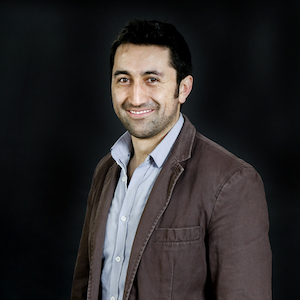
\includegraphics[width=1.35417in,height=\textheight]{Figures/Fabio.jpg}

}

\end{figure}

\end{col}

\begin{col}{0.05\textwidth}
~

\end{col}

\begin{col}{0.75\textwidth}
Franco-Colombien, Né le 06/05/1988 à Bogota, Colombie

27, Rue du Pont de Pierre, 54270 - Essey-les-Nancy

Tel : 07.78.78.38.07

\faIcon{envelope} \url{fabbiocrux.ms@gmail.com}

\faIcon{github} \href{https://github.com/fabbiocrux}{Open Science with
Github}

\aiGoogleScholar ~
\href{https://scholar.google.fr/citations?user=8Cuoaf4AAAAJ&hl=fr}{Google scholar}

CNU \textbf{60}, 62

Recyclagé distribué; 3D Printing; Recyclage plastique; Soutenabilité

\end{col}

\end{cols}

\hypertarget{pruxe9sentation}{%
\subsection{Présentation}\label{pruxe9sentation}}

Je suis ingénieur mécanique formé à l'Université Nacional de Colombie,
titulaire d'un Master II en Management de l'Innovation et du Design
Industriel et PhD. en Génie des Systèmes Industriels de l'Université de
Lorraine.

\begin{wrapfigure}{r}{0.5\textwidth}
  \begin{center}
    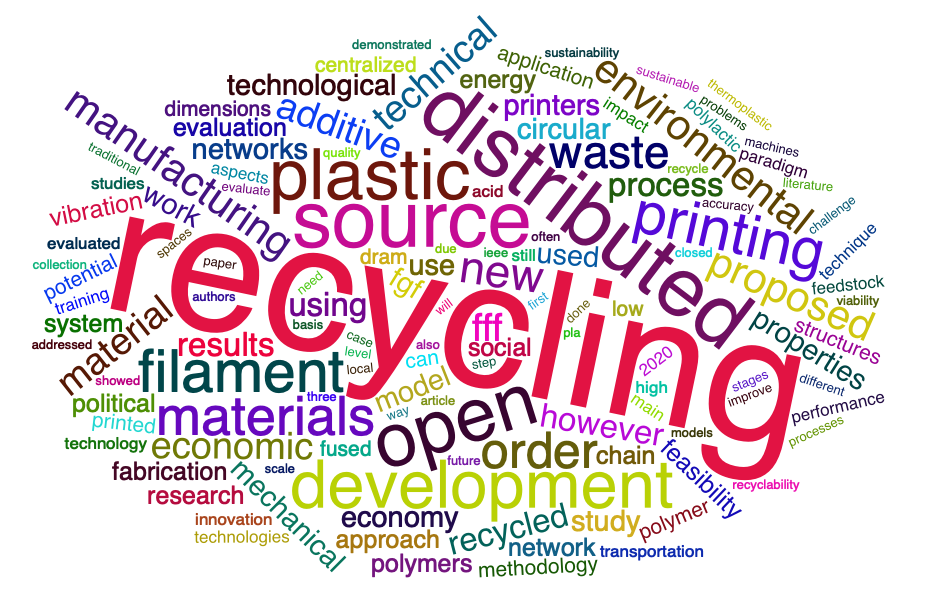
\includegraphics[width=0.48\textwidth]{Figures/Cloud.png}
  \end{center}
  \caption{Nuages de mots fait à partir des résumés des mes articles scientifiques}
\end{wrapfigure}

Mon domaine de recherche est la fabrication additive open source
(également appelé Impression 3D) comme vecteur de développement
industriel soutenable. Plus précisément, sur l'étude systémique de
nouvelles filières distribuées en circuit court pour la valorisation des
matières plastiques recyclées via la fabrication additive. Cela implique
une approche multi-échelle afin d'appréhender à la fois les enjeux liés
au procédé technologique, à la filière associée et au territoire, en
privilégiant collaborations avec de multiples acteurs et la mobilisation
de différentes méthodologies pour améliorer, tester et expérimenter de
nouveaux usages.

Mon travail se décompose en trois échelles principaux. Un premier
échelle porte sur la validation du procédé d'impression 3D open source
en tant qu'outil reproductible pour la fabrication des pièces imprimées
en thermoplastique. Une attention particulière est portée sur la
précision géométrique, résistance mécanique et vibratoire de ce procédé
à l'échelle industrielle standard. Une deuxième échelle centrale dans
mon parcours est la faisabilité technique du recyclage des
thermoplastiques pour les processus d'impression. J'ai eu l'opportunité
de travailler pendant ma thèse sur les caractérisations mécaniques et
chimiques de la matière recyclée dans la chaîne d'impression en
co-tutelle avec l'Équipe de Recherche sur les Processus Innovatifs
(ERPI) et le Laboratoire des Réactions et Génie des Procédés (LRGP ---
UMR 7274) à Nancy. Je collabore avec le groupe de recherche FAST (Free
Appropriate Sustainability Technology) de Western University de Canada
sur le développement open source hardware dans une vision de
démocratisation de la technologie associé au recyclage distribué. Une
troisième échelle en cours de développement est l'analyse de la
soutenabilité d'une filière de recyclage distribuée en collaboration
avec l'équipe InSyTe de l'Université Technologique de Troyes. Le
développement d'indicateurs (au-delà des indicateurs
technico-économiques) intégrant la capacité de charge des écosystèmes et
leurs services est un enjeu prometteur pour rendre les filières
industrielles plus résilientes.

J'ai une forte expérience en montage et conduite de projet européens.
J'ai l'opportunité de mettre en œuvre ces travaux de recherche dans le
cadre du projet H2020
\href{http://erpi.univ-lorraine.fr/projects/INEDIT/}{INEDIT} qui vise le
transfert des approches `Do-It-Yourself' (DIY) vers un contexte
industriel. Je développe donc le démonstrateur de recyclage des
plastiques pour l'impression 3D
\href{https://lf2l.fr/projects/green-fablab/}{`\emph{Green
Fablab}'}\footnote{https://lf2l.fr/projects/green-fablab/} afin de
tester l'approche appelée `Do-It-Together' (DIT). C'est une excellente
opportunité pour mieux comprendre l'opérationnalisation et la
démultiplication de la démarche de recyclage distribué auprès des
acteurs et des communautés locales. En parallèle, je pilote également
dans le projet
\href{https://erpi.univ-lorraine.fr/fr/projects/Climatelabs/}{Erasmus+
Climatelabs} qui cherche à renforcer les capacités de recherche
appliquée et d'innovation de dix universités partenaires du Mexique, du
Brésil et de la Colombie par la conception et la mise en œuvre des
espaces d'innovation sociales pour l'atténuation et l'adaptation au
changement climatique.

\hypertarget{formations}{%
\subsection{Formations}\label{formations}}

\begin{tabu} to \linewidth {X[0.3,l] X[2,l]}

2013 -- 2016 & \textbf{Ph.D., Université de Lorraine}, spécialité Génie des systèmes industriels \par
    Titre de thèse: \textbf{\emph{Methodological proposition to evaluate polymer recycling in open-source additive manufacturing contexts}} \par\vspace{5pt}
    
Défendu publiquement le 9 Décembre de 2016 à Nancy devant le jury:\par\vspace{5pt}

    \textbf{Rapporteurs:}
    \begin{itemize}
    
        \item \textit{Prof.} Nicolas PERRY --  ENSAM, Bordeaux - France
        \item \textit{Dr.} Salim BELOUETTAR -- LIST, Esch-sur-Alzette - Luxembourg
    \end{itemize}

\vspace{5pt}
    \textbf{Examinateurs:}
    \begin{itemize}
    
        \item \textit{Prof.} Joshua M. PEARCE -- MTU, Michigan - USA
        \item \textit{Prof.} Nadia BAHLOULI -- Université de Strasbourg, Strasbourg - France
        \item \textit{Prof.} Mauricio CAMARGO (\textit{Directeur}) -- UL, ERPI, Nancy - France
        
        \item \textit{MdC.} Hakim BOUDAOUD (\textit{co-directeur}) -- UL ERPI, Nancy - France
        
        \item \textit{Dr.} Sandrine HOPPE (\textit{co-directeur})  --  LRGP, Nancy - France
    \end{itemize}
        \\ [5pt]

2012 -- 2013 &
    \textbf{Master II.~ Management de l'Innovation et du Desing Industriel, Université de Lorraine, FR} \par Titre: \emph{Proposition d'un Protocole d'expérimentation standard pour la fabrication additive open source} \\[5pt]

2004 -- 2012 &
    \textbf{B.Sc. Ingénieur Mécanique}, Universidad Nacional de Colombia, Bogotá, Colombie \\
    
\end{tabu}

\hypertarget{expuxe9riences-professionnelles}{%
\subsection{Expériences
Professionnelles}\label{expuxe9riences-professionnelles}}

\extrarowsep=3pt
\begin{tabu} to \linewidth {X[0.4,l] X[2,l]}
2022 -- ... &
    \textbf{Chercheur contractuel} Université de Lorraine, Université de Lorrain, Nancy -- France \\[5pt]

2021 -- 2021 &
    \textbf{Chercheur contractuel} Université de Technologique de Troyes, Équipe InSyTe (Anciennement CREIDD) Troyes -- France \\[5pt]

2017 -- 2021 &
    \textbf{Post-doctorant} Université de Lorraine, Université de Lorrain, Nancy -- France \\[5pt]

2010 -- 2011 & \textbf{International trainee} \href{http://www.mipengenharia.com.br/}{Entreprise MIP Engenharia S/A} \thinspace Belo Horizonte, Brazil \par
\textit{Projet:} Aide à la création d'un plan stratégique pour le projet d'internationalisation de MIP. Développement d'un benchmarking d'entreprises ayant un profil commercial similaire sur les marchés chilien, colombien et péruvien. \\
    
2008 -- 2009 &
    \textbf{Étudiant adjoint ingénieur} \emph{Universidad Nacional de Colombia. Bogotá - Colombia}  \par 
    \emph{Projet:} Conception et construction d'une machine de coulée centrifuge pour la fabrication de cylindres en fonte ASTM 40. \\
\end{tabu}

\hypertarget{compuxe9tences}{%
\subsection{Compétences}\label{compuxe9tences}}

\extrarowsep=3pt
\begin{tabu} to \linewidth {X[0.1,l] X[2,l]}

\faIcon{language}  & 

\includegraphics[width=2ex]{Figures/icons/flag-colombia.png} Langue Maternelle\quad 

\includegraphics[width=2ex]{Figures/icons/flag-france.png} Courante  \quad
\includegraphics[width=2ex]{Figures/icons/flag-usa.png} Courante  \quad
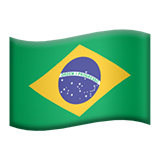
\includegraphics[width=2ex]{Figures/icons/flag-brazil.png} Professionnel \\[5pt] 


\faIcon{laptop}  & CAO (Solid-Works, Onshape), Matlab,  Data analysis / visualization, R, \textsc{Html, css} \\[5pt]
    

\faIcon{book}  & Academic research,  Mendeley, \LaTeX ~and Rmarkdown publishing.

\end{tabu}

\hypertarget{activituxe9s-de-recherche}{%
\section{Activités de Recherche}\label{activituxe9s-de-recherche}}

\hypertarget{synthuxe8se-quantitative}{%
\subsection{Synthèse quantitative}\label{synthuxe8se-quantitative}}

Sur la période 2014-2023, 9 articles dans des revues internationales à
comité de lecture et 6 conférences internationales ont été publiés comme
illustré dans la Figure~\ref{fig-bilan}. Cette production scientifique
relève de mes travaux de recherche dans les différentes échelles
auxquelles je développe mon domaine d'investigation au sein du
laboratoire ERPI.

Au cours de l'année 2023, 3 propositions d'articles ont été soumis dans
des revues à comité de lecture (en attente de décision) et 2 chapitres
d'ouvrages collectifs à destination de la communauté du recyclage des
matériaux sont en cours de révision par les éditeurs. Le tableau montre
les différents journaux dans lesquels nos propositions ont été publiées.
L'annexe A présente une liste complète de la production scientifique.

\begin{figure}[H]

{\centering 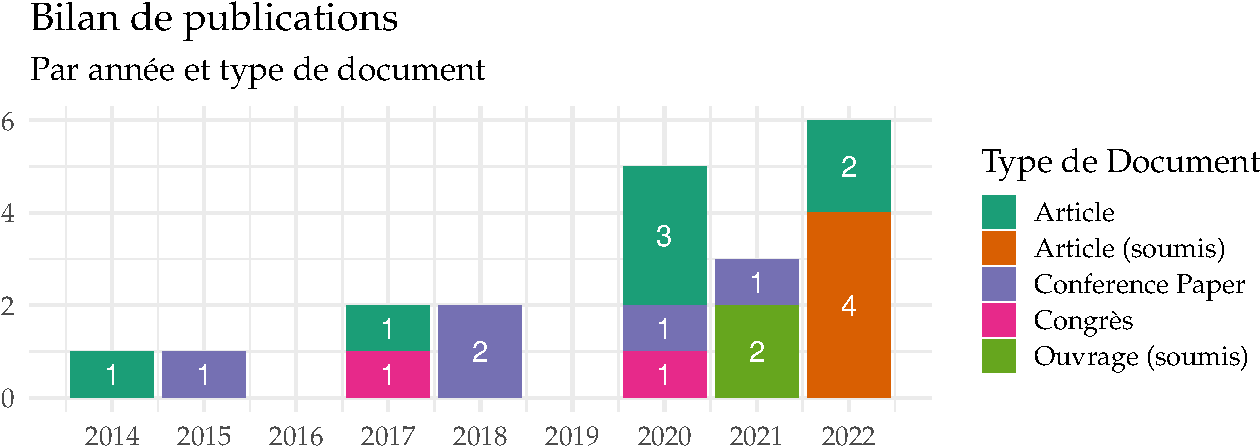
\includegraphics[width=0.95\textwidth,height=\textheight]{Figures/fig-bilan-1.pdf}

}

\caption{\label{fig-bilan}Bilan de production scientifique}

\end{figure}

\begin{small}
\begin{minipage}{0.6\linewidth}

\begin{tabu} to \linewidth {X[2,l] X[0.5,l]}
\toprule
\textbf{Journaux} & \textbf{IF (2020)} \\
\midrule
\href{https://www.journals.elsevier.com/additive-manufacturing}{Additive Manufacturing} & 10.998 \\
\href{https://www.journals.elsevier.com/resources-conservation-and-recycling}{Resources, Conservation \& Recycling} & 10.204\\

\href{https://www.journals.elsevier.com/journal-of-cleaner-production}{Journal of Cleaner Production} &  9.297\\
\href{https://www.tandfonline.com/toc/nvpp20/current}{Virtual and Physical Prototyping}
 & 8.092\\

\href{https://home.liebertpub.com/publications/3d-printing-and-additive-manufacturing/621/overview}{3D Printing and Additive Manufacturing}
 & 5.449\\
 
\href{https://www.springer.com/journal/11837}{JOM} & 2.474 \\
\href{https://www.journals.elsevier.com/cleaner-engineering-and-technology}{Cleaner Engineering and Technology} & -- \\

\href{https://journals.sagepub.com/home/pib}{Proceedings of the Institution of Mechanical Engineers, Part B: Journal of Engineering Manufacture} & 2,759 \\

\bottomrule
\end{tabu}
\end{minipage}
\quad
\begin{minipage}{0.40\linewidth}
\begin{tabu} to \linewidth {X[0.2,c] X[2.5,l]}
\toprule
 & \textbf{Conferences et congrès} \\
\midrule
3 & Communications dans des conférences internationales en ingénierie et management de la technologie (ICE/IEEE) \\
3  & Communications conferences sur la fabrication additive (Solid
Freeform Fabrication Symposium)  \\
1 & Participation aux congrès de la Société française de génie des procédés (SFGP) \\
1 & Participation à summer school (spring of innovation and circular economy) \\
\bottomrule
\end{tabu}
\end{minipage}
\end{small}

\hypertarget{synthuxe8se-qualitatif-des-mes-axes-de-recherche}{%
\subsection{Synthèse qualitatif des mes axes de
recherche}\label{synthuxe8se-qualitatif-des-mes-axes-de-recherche}}

\begin{tcolorbox}[enhanced jigsaw, toprule=.15mm, bottomtitle=1mm, toptitle=1mm, rightrule=.15mm, title=\textcolor{quarto-callout-tip-color}{\faLightbulb}\hspace{0.5em}{En quelque mots}, arc=.35mm, opacityback=0, titlerule=0mm, breakable, colframe=quarto-callout-tip-color-frame, colback=white, colbacktitle=quarto-callout-tip-color!10!white, opacitybacktitle=0.6, left=2mm, leftrule=.75mm, bottomrule=.15mm, coltitle=black]

Mes travaux de recherche portent sur l'étude systémique multi-echelle
(produit / procédé / filière / territoire) de nouvelles filières
distribuées en circuit court pour la valorisation des matières
plastiques recyclées via la fabrication additive.

\end{tcolorbox}

La particularité de la recherche que je développe au sein du laboratoire
ERPI est de mieux comprendre le système technologique du processus de
recyclage que l'impression 3D open source est en train de rendre
factible. L' enjeu sociétal majeur est de pouvoir décrire, modéliser,
opérationnaliser et évaluer un système productif et de revalorisation
des déchets de façon locale et distribuée. Les statistiques sur la
problématique de déchets plastiques font preuve que d'autres approches
au-delà de la centralisation et de l'économie d'échelle doivent être
explorées. Donc, l'étude sur la notion distribué, sur sa dimension
opérationnelle du système, et également l'implication systémique de
cette nouvelle filière pour un territoire en identifiant un ensemble
d'indicateurs multicritères afin d'évaluer cette type de propositions
est un gap dans la littérature scientifique auquel je travaille pour
donner.

Mes activités de recherche ont un fort lien avec la plateforme de
recherche du Lorraine Fab Living Lab, car depuis quelques années, il y a
une interet croissance sur les espaces d'innovation ouverte type Fab
Labs / hackerspaces. Ces types des espaces sont un levier fort de
démultiplication de capacités de production distribué, dont le vecteur
industriel de la fabrication additive s'y déploies de façon inhérente.
Ces types d'espaces démocratisent les processus de prototypage et de
matérialisation des idées.

Mes travaux de recherche ont abouti à une proposition de cadre
conceptuel pour le déploiement d'une filière de recyclage des
thermoplastiques pour l'impression 3D en considérant les étapes clés
comme illustré dans la Figure~\ref{fig-sdram}.

\begin{figure}[H]

{\centering 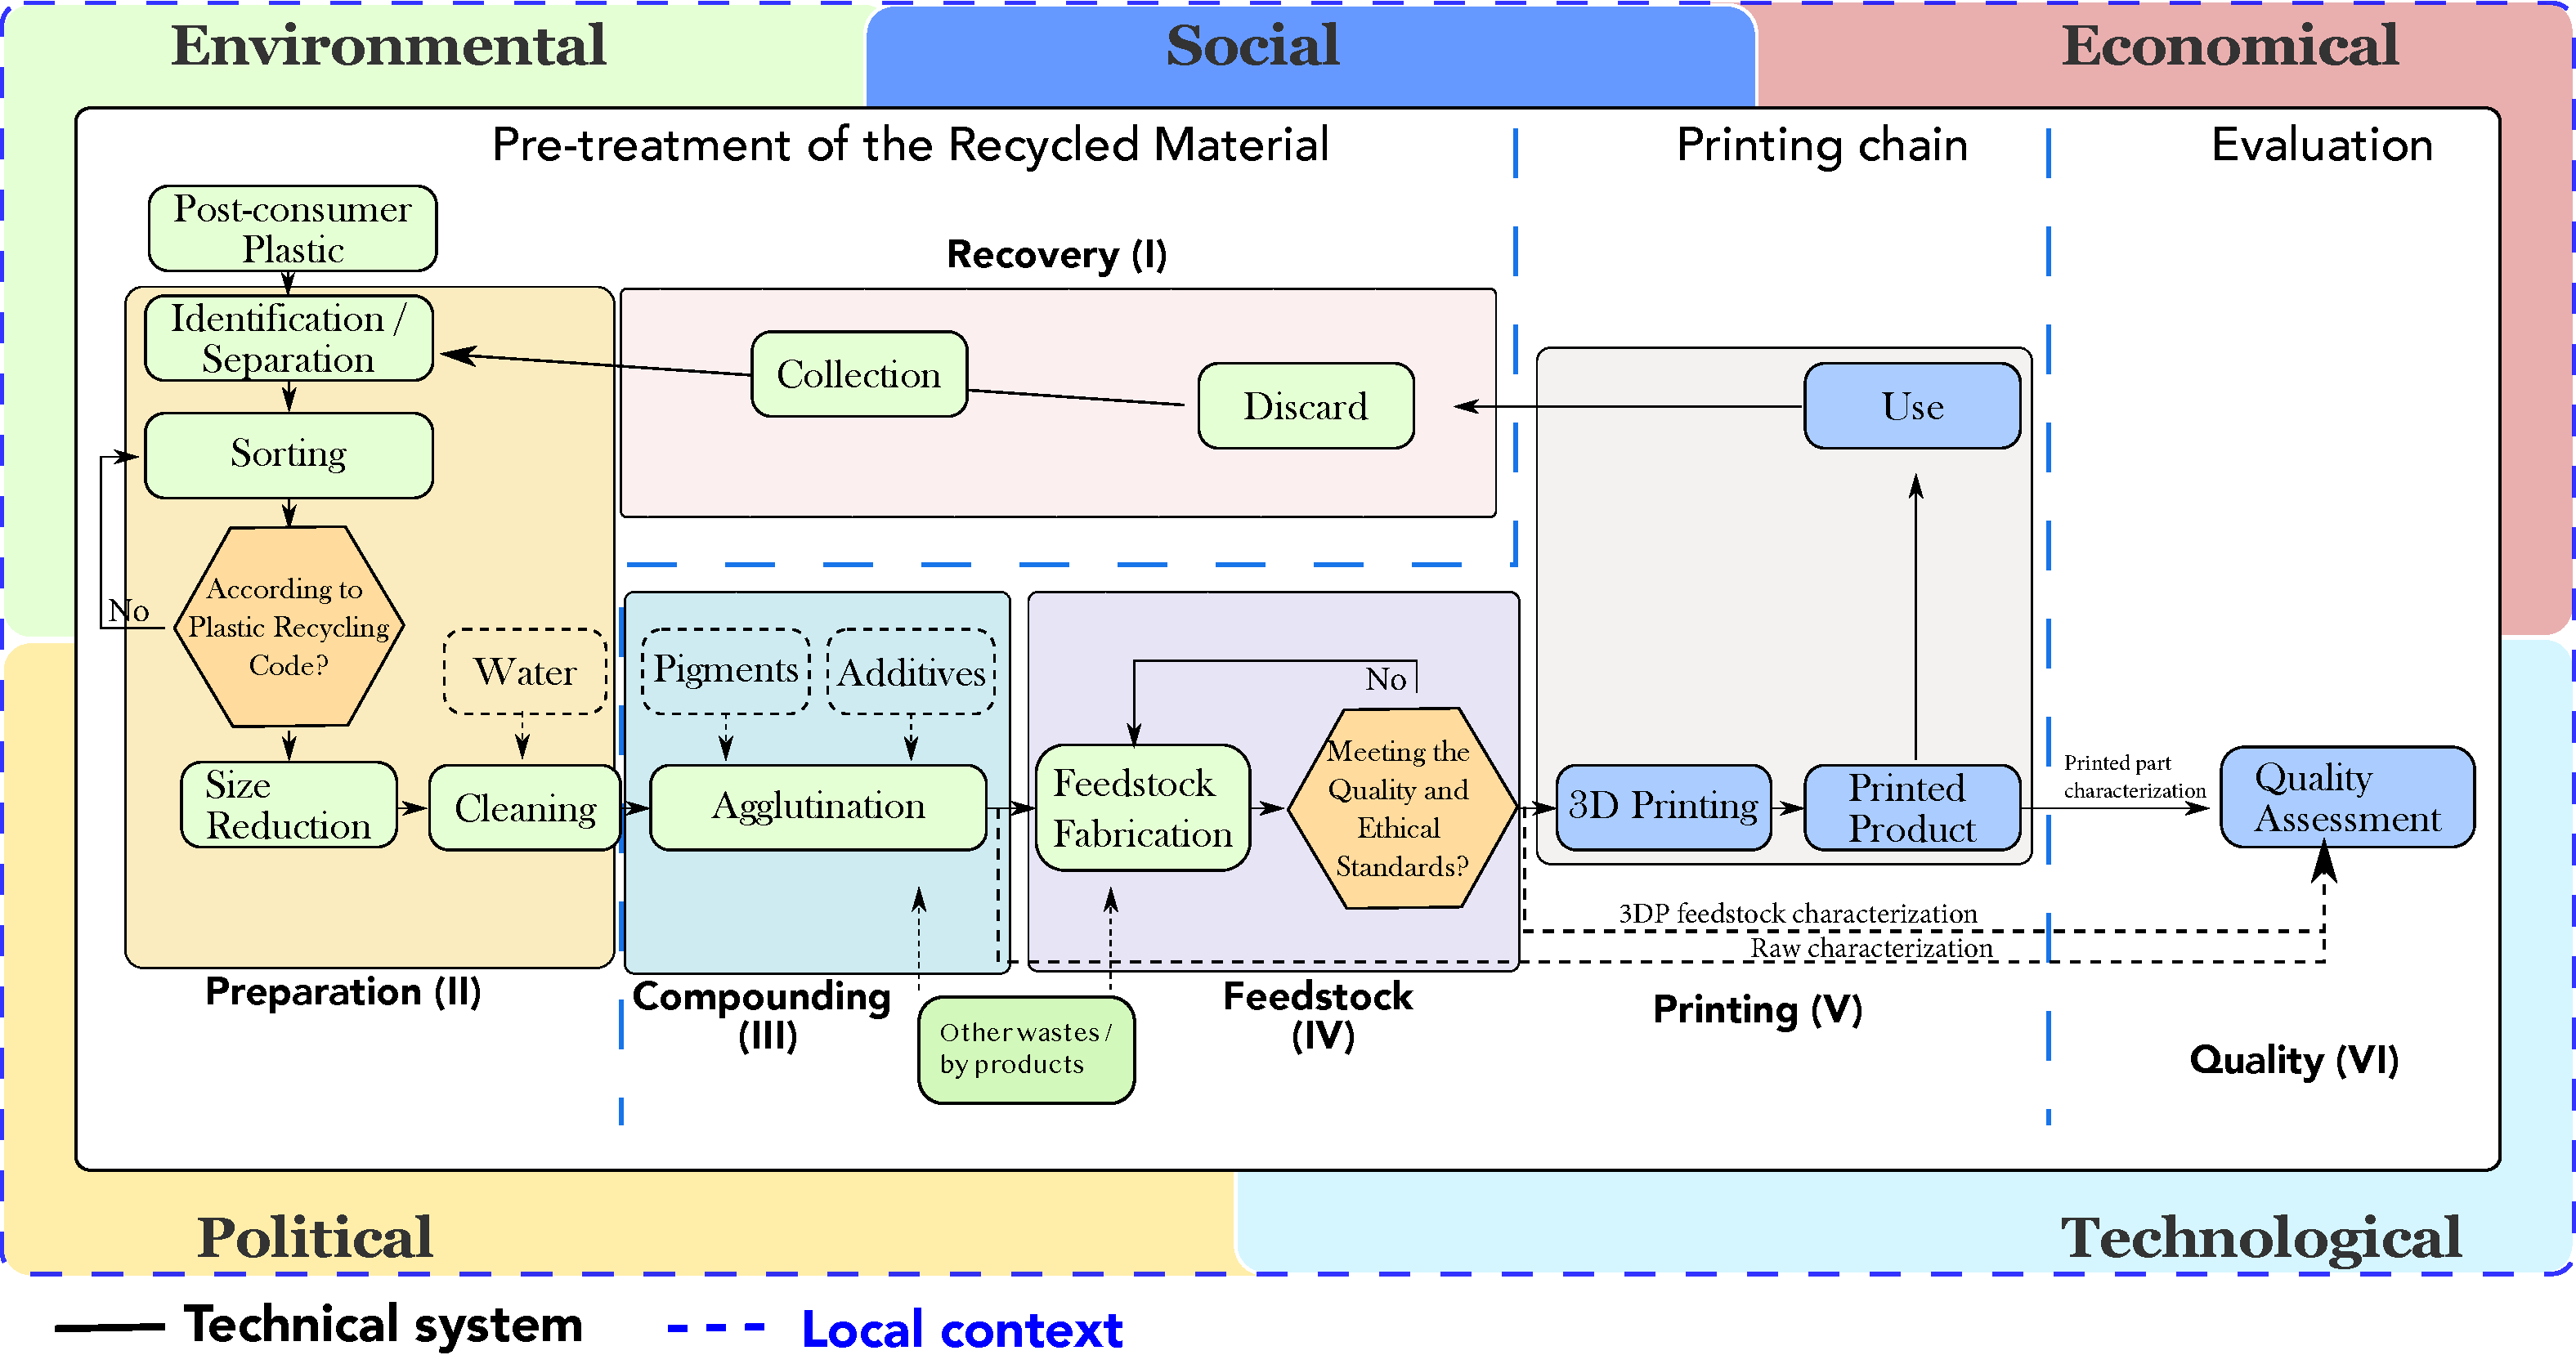
\includegraphics[width=0.9\textwidth,height=\textheight]{Figures/SDRAM-00.pdf}

}

\caption{\label{fig-sdram}Récyclage distribué via la fabrication
additive}

\end{figure}

Je travaille au sein du laboratoire ERPI avec différents collègues en
France et à l'étranger pour pouvoir clarifier étape par étape (I-VI) les
implications, les verrous scientifiques et technologiques afin de
démocratiser une démarche locale de recyclage distribuée. Chaque élément
est très important, notamment dans un contexte où la société doit agir à
tous les niveaux (produit-procédé / filière / territoire) vers une
transition écologique des modes de production, de fabrication et de
consommation en prenant en compte les enjeux environnementaux actuels.

Actuellement, dans le cadre du projet INEDIT, qui vise le transfert des
approches `Do-It-Yourself' vers un context industriel, nous sommes en
train de mettre en place un démonstrateur qui permettra de tester
l'approche appelé `Do-It-Together' dont la particularité consiste à
coupler les phases de co-création et conception produit avec une notion
de fabrication ouverte grâce à des plateformes numériques en incluant la
réalité virtuelle (Figure~\ref{fig-DRAM-INEDIT}).

\begin{figure}[H]

{\centering 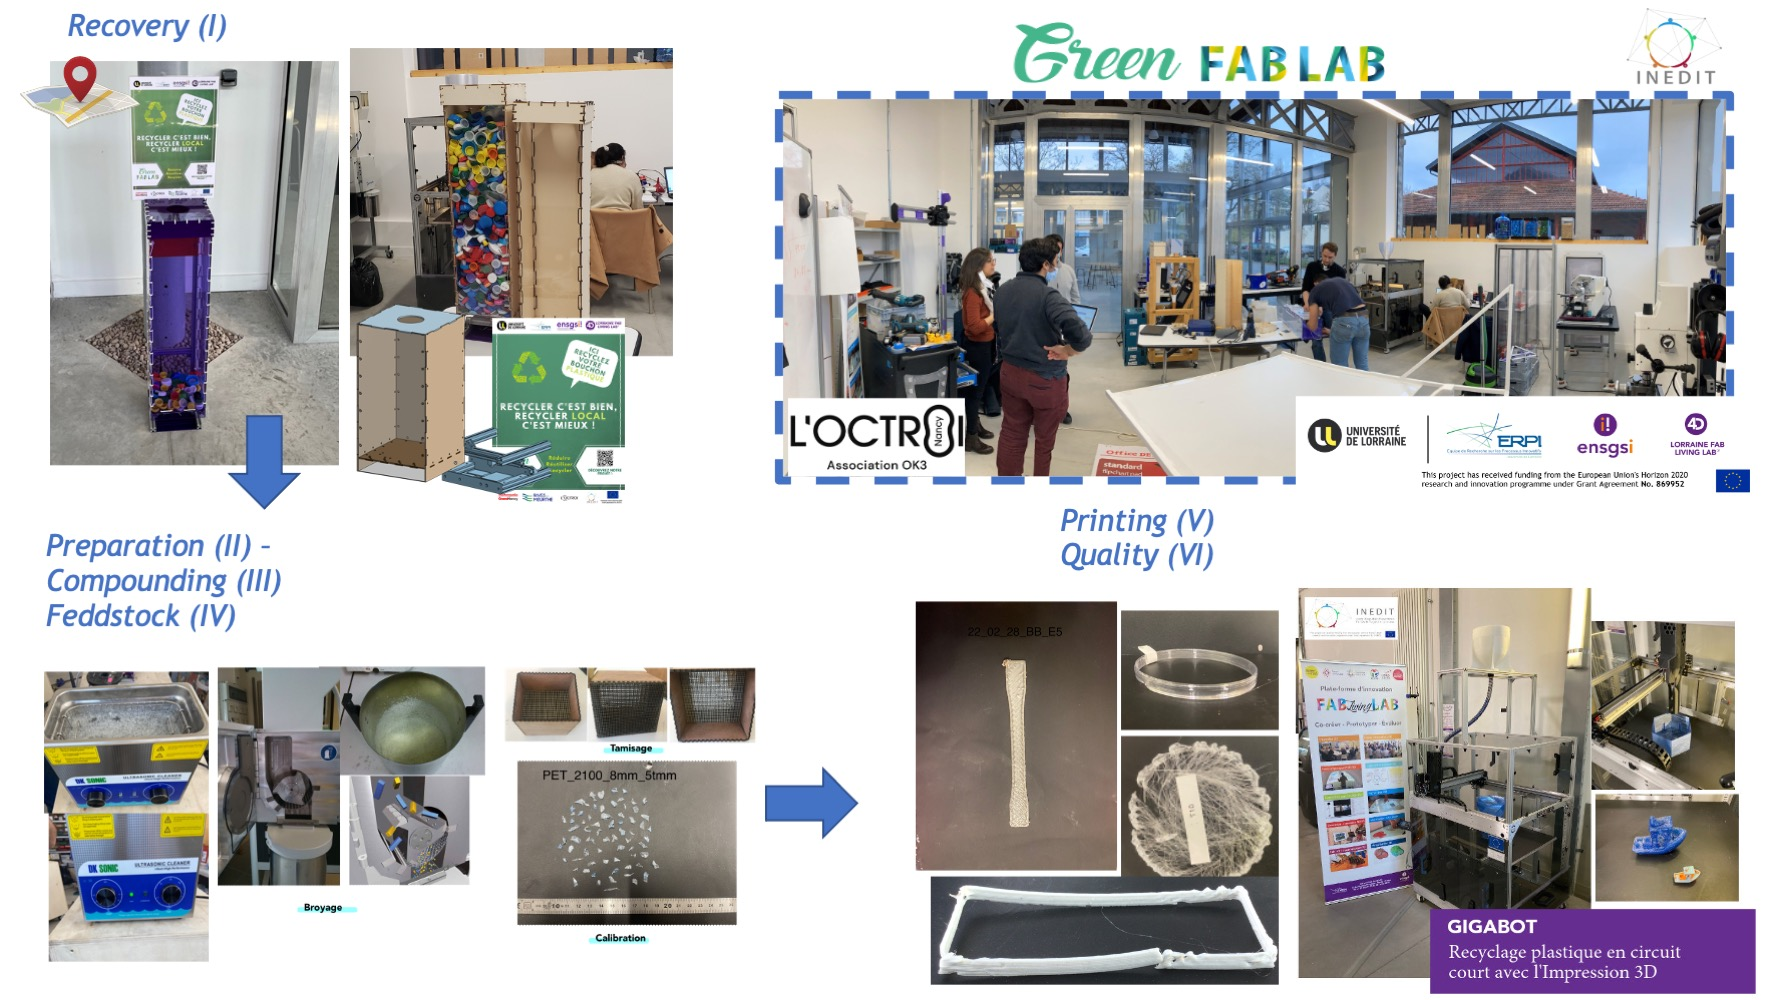
\includegraphics[width=0.9\textwidth,height=\textheight]{Figures/INEDIT.jpg}

}

\caption{\label{fig-DRAM-INEDIT}Récyclage distribué via la fabrication
additive}

\end{figure}

Le développement de ce projet mobilise un panel de méthodologies de
recherche dans la conception mécanique (e.g: plan d'expériences,
validation statistique/ANOVA, simulation) et en innovation
(e.g.~recherche opérationnelle, analyse multicritère, systèmes
dynamiques) en ouvrant un champ d'expérimentation non négligeable pour
la créativité de solutions avec des étudiants en ingénierie.

A partir de ce contexte, les axes de recherche peuvent être décrits d'un
point de vue technologique (micro) vers une vision système (macro) de
l'implication de la filière de recyclage en tant que système
socio-technique.

\hypertarget{limpression-3d-open-source-validation-des-standards-de-fabrication}{%
\subsubsection{L'impression 3D open source: validation des standards de
fabrication}\label{limpression-3d-open-source-validation-des-standards-de-fabrication}}

La fabrication additive est reconnue comme un sujet disruptif. Elle est
en train de changer les repères technologiques des domaines industriels,
de la conception et du design, mais aussi à une échelle globale dans la
société. Le principe de la fabrication couche-par-couche offre un nouvel
espace de liberté pour la conception mécanique et la fabrication grâce à
une meilleure maîtrise de l'apport en matière première.

La technologie de dépôt de fil fondu (Fused Filament Fabrication --FFF-
en anglais) est la plus répandue grâce à son principe d'extrusion de
polymère qui offre une grande flexibilité. Sa démarche de conception
open source permet un processus collaboratif d'amélioration distribué à
moindre coût. Cependant, la démultiplication des types de machines, des
matériaux utilisés et des expérimentations appellent à la détermination
de standards de performances permettant ainsi une comparaison et une
validation des procédés techniques.

Une première échelle d'analyse sur laquelle je travaille concerne la
validation des procédés open source en tant qu'outil de fabrication
reproductible et fiable pour un usage semi-industriel J'ai eu
l'opportunité de me concentrer sur la caractérisation de la performance
géométrique à travers des modèles de benchmarking\footnote{\textbf{Cruz
  Sanchez, F.A.}, Boudaoud, H., Muller, L., Camargo, M., 2014. Towards a
  standard experimental protocol for open source additive manufacturing.
  Virtual Phys. Prototyp. 9, 151--167.
  https://doi.org/10.1080/17452759.2014.919553}, des expérimentations
pour des applications médicales\footnote{Albuquerque, R., Arbelaez, G.,
  \textbf{Cruz, F.}, Camargo, M., Joseph, D., Tran, N., 2018. Modelling,
  Printing and Validation of Dental Dry Models for Implantology Skills
  Training, in: 2018 IEEE International Conference on Engineering,
  Technology and Innovation (ICE/ITMC). IEEE, pp.~1--8.
  https://doi.org/10.1109/ICE.2018.8436302} où j'ai exploré le
comportement mécanique des matériaux. Systématiquement, des plans
d'expériences et d'analyses statistiques ont été mis en œuvre grâce à la
mobilisation de méthodologies adaptées. Nous explorons également le
comportement vibratoire et d'amortissement des échantillons à partir de
FFF\footnote{Xue, F., Robin, G., Boudaoud, H., \textbf{Cruz Sanchez,
  F.A.}, Daya, E.M., 2022. General Methodology to Investigate the Effect
  of Process Parameters on the Vibration Properties of Structures
  Produced by Additive Manufacturing Using Fused Filament Fabrication.
  JOM 74, 1166--1175. https://doi.org/10.1007/s11837-021-05051-9} avec
les collègues du Laboratoire d'Études des Microstructures et de
Mécanique des Matériaux (LEM3) à Metz - France. Ces travaux permettent
de positionner la FFF open source auprès de la communauté scientifique
et industrielle en tant qu'outil fiable et reproductible.

D'un autre côté, le procédé de dépôt par granulés (Fused Granular
fabrication --FGF- en anglais) est une avancée technologique récente et
représente une grande opportunité dans la démocratisation de
l'impression 3D. Ce procédé utilise directement de la matière première
en forme de pellet. Cela ouvre un champ d'exploration afin de faciliter
l'impression de grande taille pour des matériaux élastomères
thermoplastiques et de matière composites. J'ai pu entamer un travail de
comparaison de procédé FGF avec le FFF dans la performance
mécanique\footnote{Alexandre, A., \textbf{Cruz Sanchez, F.A.}, Boudaoud,
  H., Camargo, M., Pearce, J.M., 2020. Mechanical Properties of Direct
  Waste Printing of Polylactic Acid with Universal Pellets Extruder:
  Comparison to Fused Filament Fabrication on Open-Source Desktop
  Three-Dimensional Printers. 3D Print. Addit. Manuf. 3dp.2019.0195.
  https://doi.org/10.1089/3dp.2019.0195}. Cependant, le défi actuel
réside dans une meilleure compréhension de la communauté scientifique
des caractéristiques du procédé au sens précision dimensionnelle,
imprimabilité des matériaux et faisabilité économique de cette
technologie.

\hypertarget{filiuxe8re-durable-de-limpression-3d-pour-le-ruxe9cyclage}{%
\subsubsection{Filière durable de l'impression 3D pour le
récyclage}\label{filiuxe8re-durable-de-limpression-3d-pour-le-ruxe9cyclage}}

Une deuxième échelle de ma recherche concerne la proposition d'une
méthodologie systématique permettant d'évaluer la fabrication et
l'évaluation de la matière recyclée utilisée dans le procédé
d'impression. Cette méthodologie facilite l'étude et la modélisation
d'une filière de recyclage en circuit court pour l'impression 3D open
source.

L'enjeu essentiel de ma thèse et de mon projet de post-doc 2017-2019 a
été de démontrer l'imprimabilité des matières recyclées. En ce sens,
j'ai réalisé le couplage de tests de caractérisation des propriétés
mécaniques (e.g.~résistance à la traction, module d'élasticité) et
chimiques (e.g viscosité, calorimétrie) avec de multiples cycles
d'extrusion, impression et de moulage par injection. L'un de mes
premiers résultats est une démarche de caractérisation
chimique\footnote{\textbf{Cruz, F.}, Lanza, S., Boudaoud, H., Hoppe, S.,
  Camargo, M., 2015. Polymer Recycling and Additive Manufacturing in an
  Open Source context : Optimization of processes and methods, in: Solid
  Freeform Fabrication. Austin, Texas, pp.~1591--1600.}, et mécanique
\footnote{\textbf{Cruz Sanchez, F.A.}, Boudaoud, H., Hoppe, S., Camargo,
  M., 2017. Polymer recycling in an open-source additive manufacturing
  context: Mechanical issues. Addit. Manuf. 17, 87--105.
  https://doi.org/10.1016/j.addma.2017.05.013} de la dégradation de
l'acide polylactique (PLA) qui est le thermoplastique le plus utilisé
dans le domaine FFF. Mon travail de thèse a eu pour résultat principal
de montrer que le recyclage distribué du plastique à l'aide de
technologies 3D open source (imprimantes 3D et extrudeuses) est une
option possible pour la valorisation des déchets plastiques. Cette
approche pour évaluer la recyclabilité permet de simuler le cycle de vie
prolongé des produits recyclés.

D'autre part, au vu des ces résultats encourageants, j'ai eu
l'opportunité d'accompagner les travaux de thèse de Pavlo Santander
pendant la période 2017-2020. Nous avons donc changé de perspective dans
le but de prouver la faisabilité de recyclage au niveau de la chaîne
d'approvisionnement afin de mieux comprendre les paramètres logistiques
liés à cette filière de recyclage.

Le faible taux actuel de recyclage des plastiques montre les limites de
l'approche actuelle de gestion centralisée des déchets. Ce processus
centralisé est complexe, coûteux et polluant en raison des multiples
étapes de tri, de collecte et de transport. Le recyclage distribué des
plastiques peut être imaginé comme une sorte de ``réseau intelligent'',
composé de petites unités de recyclage coordonnées fournissant des
matières premières secondaires (eg: filaments recyclés) à une communauté
(e.g.~collèges / lycées, espaces fablabs et de prototypage). Le modèle
conceptuel\footnote{Pavlo, S., \textbf{Fabio, C.}, Hakim, B., Mauricio,
  C., 2018. 3D-Printing Based Distributed Plastic Recycling: A
  Conceptual Model for Closed-Loop Supply Chain Design, in: 2018 IEEE
  International Conference on Engineering, Technology and Innovation
  (ICE/ITMC). IEEE, pp.~1--8. https://doi.org/10.1109/ICE.2018.8436296},
et son application dans le contexte de Nancy en lien avec le projet
Green Fablab\footnote{Santander, P., \textbf{Cruz Sanchez, F.A.},
  Boudaoud, H., Camargo, M., 2020. Closed loop supply chain network for
  local and distributed plastic recycling for 3D printing: a MILP-based
  optimization approach. Resour. Conserv. Recycl. 154, 104531.
  https://doi.org/10.1016/j.resconrec.2019.104531} ont prouvé son
approche originale et une mise en œuvre reproductible.

Cette nouvelle approche du recyclage propose un système local adapté aux
petites quantités de déchets. Sous ce nouveau paradigme, les problèmes
économiques et environnementaux d'un recyclage centralisé seraient
limités, principalement en raison de l'utilisation d'une technologie
open source moins coûteuse, de plus courtes distances entre le lieu de
récupération et le point de traitement.

Cet axe est en cours de recherche, et fait l'objet du développement dans
le projet de démonstration appliqué INEDIT.

\hypertarget{espace-dinnovation-pour-la-circularituxe9}{%
\subsubsection{Espace d'innovation pour la
circularité}\label{espace-dinnovation-pour-la-circularituxe9}}

La troisième échelle porte sur la compréhension des espaces d'innovation
comme un levier fort pour l'intégration de projets locaux participatifs,
dans notre cas, la création d'une filière de recyclage plastique. Les
espaces d'innovation sont un sujet de profond intérêt pour les
industriels et les académiques car ces espaces permettent de développer
des compétences d'innovation participative et de créativité collective
ainsi que de nouvelles pratiques de travail reposant sur des approches
de collaboration, de co-conception, de co-production et de co-création.

J'ai pu travailler en collaboration avec l'École d'ingénieur du CESI sur
la façon dont un projet de recyclage pédagogique est développé au sein
du laboratoire d'innovation en observant l'évolution des intentions
stratégiques du projet et du laboratoire d'innovation \footnote{Roux-Marchand,
  T., \textbf{Cruz, F.}, Dupont, L., Camargo, M., Osorio, F., 2020.
  Connecting the strategic intent of innovation labs and projects: the
  case of the Green Fablab, in: 2020 IEEE International Conference on
  Engineering, Technology and Innovation (ICE/ITMC). IEEE, pp.~1--10.
  https://doi.org/10.1109/ICE/ITMC49519.2020.9198320}. Les impacts
tangibles et intangibles ont été mis en évidence dans la manière dont
ils se répercutent sur le pilotage d'un projet d'innovation avec des
élèves ingénieurs. Cette recherche exploratoire représente un axe de
travail intéressant pour le développement mettre en évidence l'aspect
multidisciplinaire qu'implique

Ainsi, dans une échelle européen de partage d'expériences et de
renforcement de capacités de recherche, je pilote le projet
\href{https://erpi.univ-lorraine.fr/fr/projects/Climatelabs/}{Erasmus+
Climatelabs} dont l'enjeu essentiel est de concevoir et mettre en œuvre
des espaces d'innovation avec 10 partenaires de l'Amérique latine (5 en
Colombie, 3 au Brésil et 2 Mexique). Chaque université met en œuvre un
projet pilote en fonction des leurs besoins, forces et défis locaux et
des caractéristiques des institutions de leur propre territoire. Ce
projet est une opportunité pour partager la connaissance et l'expérience
que ERPI/ENSGSI a mûri lors de la création et du développement du projet
de Green Fablab. Les notions de ``fabrication personnelle'', de
pratiques Do-It-Yourself ou de ``making'' sont souvent des approches
sociales et collaboratives, impliquant le partage et la modification de
conceptions en ligne, la coopération sur des projets et/ou l'utilisation
d'outils dans des espaces partagés. En conséquence, ces terrains
d'expérimentations en conception (mécanique et des systèmes
socio-techniques) pour chercheur et pour étudiants ingénieur prennent
tout leur sens.

\hypertarget{projet-de-recherche}{%
\subsection{Projet de recherche}\label{projet-de-recherche}}

La fabrication additive va jouer un rôle très important dans le devenir
de notre société en tant qu'outil pour la soutenabilité
(\protect\hyperlink{ref-Despeisse2016}{Despeisse et al., 2017}). Cette
technologie permet d'avoir une utilisation efficiente de la matière
première par rapport aux technologies traditionnelles de fabrication. Le
principe de dépôt couche-par-couche fait que les procédés de
l'impression 3D peuvent avoir un impact environnemental réduit en
considérant le ratio du dépôt de matière, le type de matière et la
géométrie optimisée pour l'usage adéquat. Dans le contexte du recyclage
de matière première, (dans mon cas, le recyclage de polymères
spécifiquement), la FA est une voie de recherche fondamentale pour
explorer de nouvelles méthodes d'éco-conception à multiples échelles
(\protect\hyperlink{ref-Wu2021a}{Wu et al., 2022}).

\begin{figure}[H]

{\centering 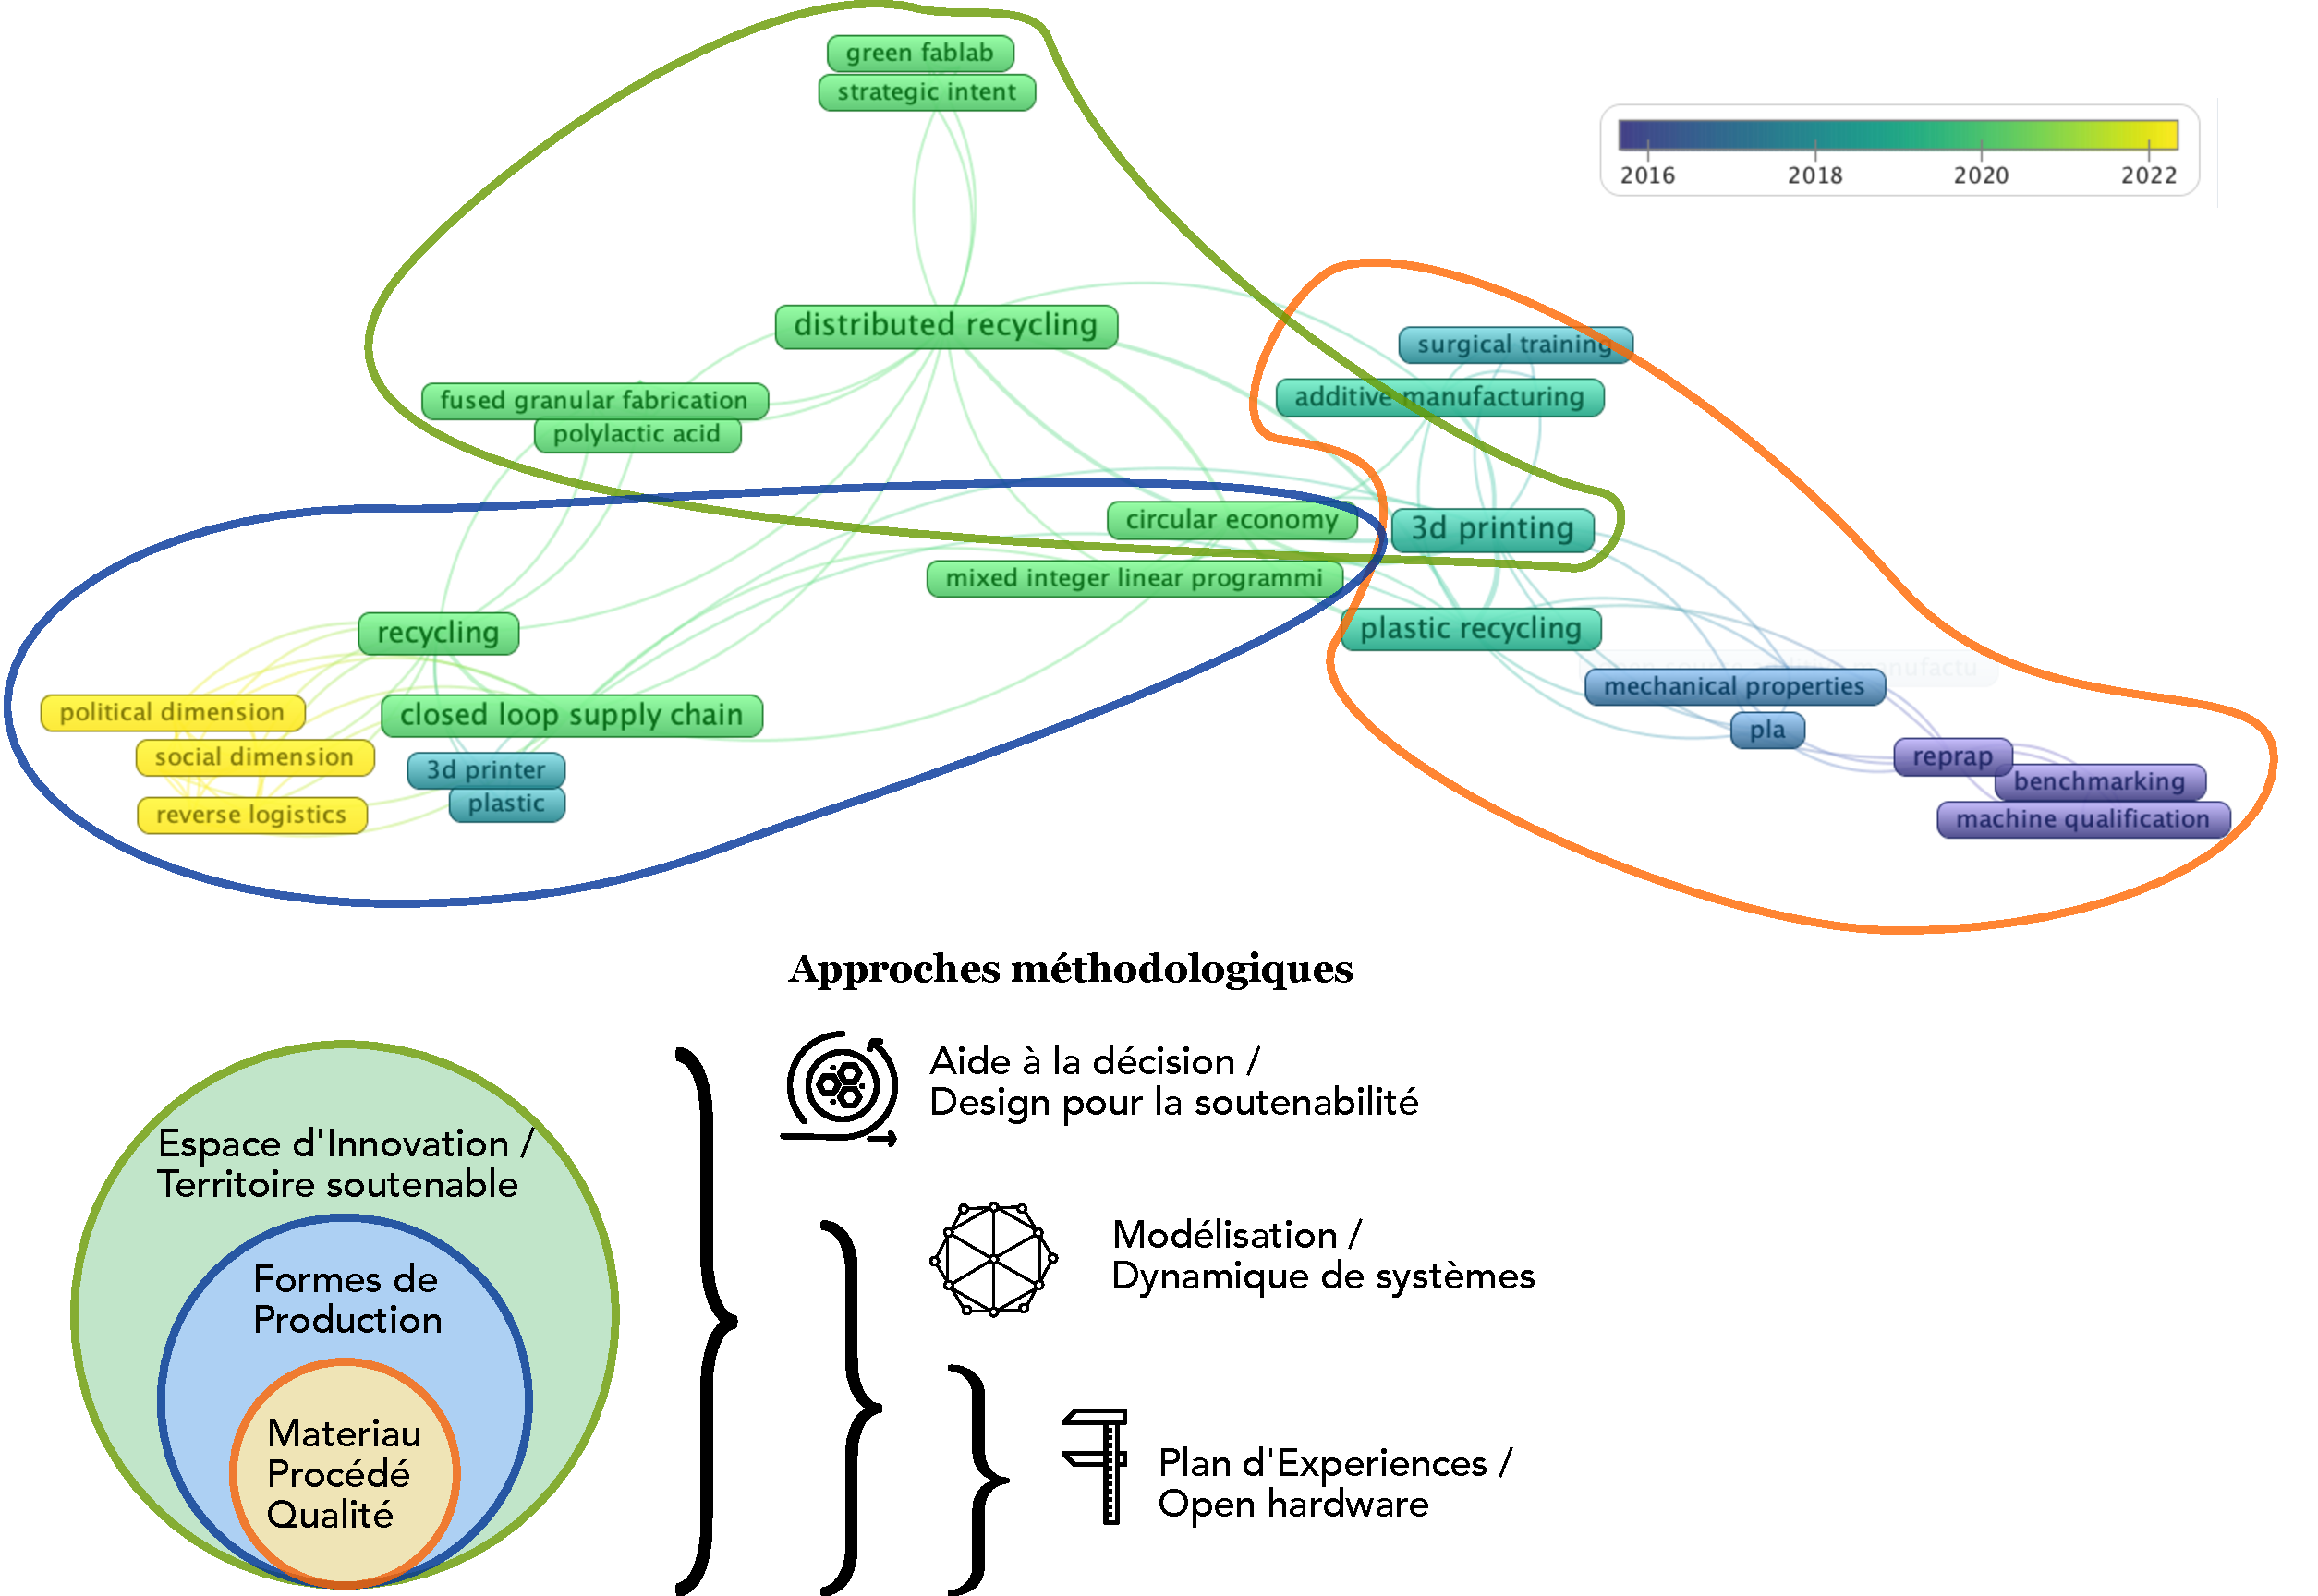
\includegraphics[width=0.9\textwidth,height=\textheight]{Figures/Vosviewer/Vosviewer-Fabio.pdf}

}

\caption{Réseau d'occurrence des mots-clés associés aux publications
(articles + conférences internationales) et évolution dans le temps}

\end{figure}

Figure @ref(fig:vosviewer) présente carte obtenue en recherchant les
mots-clés de ma recherche à l'aide du logiciel VOSviewer avec la
temporalité. En partant de cette base, le projet de recherche que je
visualise aujourd'hui concerne trois éléments importants:

\begin{enumerate}
\def\labelenumi{\arabic{enumi}.}
\tightlist
\item
  La validation des matières premières (secondaires), des procédés open
  source et de l'application de la valeur ajoutée.
\item
  L'évaluation systémique de nouvelle formes de production robustes.
\item
  Vers une soutenabilité forte pour la fabrication additive
\end{enumerate}

Le but à long terme est d'inscrire cette démarche dans l'ambition du
plan d'action de l'économie circulaire de l'Union Européenne afin de
répondre aux enjeux sociétaux de la gestion des déchets plastiques.

\hypertarget{validation-des-matiuxe8res-premiuxe8res-secondaires-procuxe9duxe9s-open-source-et-applications}{%
\subsubsection{Validation des matières premières secondaires, procédés
open source et
applications}\label{validation-des-matiuxe8res-premiuxe8res-secondaires-procuxe9duxe9s-open-source-et-applications}}

La validation de la faisabilité technique de recyclage a été faite pour
l'acide polylactique (PLA) qui est la matière la plus utilisée dans ce
domaine. Cependant, d'autres types de matériaux doivent être évalués et
caractérisés en incluant leurs applications.

Du point de vue technique, il est nécessaire de développer une
ingénierie de conception et de fabrication utilisant l'approche open
source/hardware (\protect\hyperlink{ref-Pearce2020a}{Pearce, 2020},
\protect\hyperlink{ref-Pearce2017b}{2017}) afin de promouvoir des
technologies low-cost (\protect\hyperlink{ref-Heikkinen2020a}{Heikkinen
et al., 2020}). Pour continuer à démocratiser un recyclage distribué
fiable, il faut assurer l'identification, la séparation et le nettoyage
des niches de gisements traités localement. Afin de concevoir des
produits et des systèmes qui répondent à des besoins ponctuels pour
valoriser des niches de recyclage qui n'ont pas de valorisation dans le
processus traditionnel.

\hypertarget{validation-systemique-de-nouvelle-formes-de-production}{%
\subsubsection{Validation systemique de nouvelle formes de
production}\label{validation-systemique-de-nouvelle-formes-de-production}}

L'impression 3D est une brique technologique très importante pour la
conception de nouvelles formes de production distribuée
(\protect\hyperlink{ref-Herrmann2020}{Herrmann et al., 2020} ;
\protect\hyperlink{ref-Kleer2019}{Kleer and Piller, 2019}) et pour les
technologies de l'industrie 4.0.
(\protect\hyperlink{ref-Culot2020}{Culot et al., 2020}). Ce changement
dans la façon de fabriquer conduit au besoin de développer de nouvelles
méthodes d'analyse des configurations industrielles. L'acceptabilité du
processus de recyclage distribué et sa diffusion plus importante passe
par l'identification des leviers technologiques et de leur intégration
dans les politiques publiques et sociales. Du point de vue
méthodologique, je suis intéressé par l'analyse systémique des démarches
de conception pour la soutenabilité. Ces démarches peuvent se placer au
niveau du produit, du produit-service, et aller jusqu'aux systèmes
socio-techniques (\protect\hyperlink{ref-Ceschin2016}{Ceschin and
Gaziulusoy, 2016}).

En vue de favoriser des symbioses industrielles dans une échelle micro
et meso (e.g.~éco-quartier) nous pouvons envisager plusieurs pistes
telles que la co-création avec l'utilisateur final de produits intégrant
de la matière recyclée ou la conception d'une diversité technologique
(e.g.~pas que l'impression 3D) pour la valorisation de matières
recyclées. Cependant, il faut identifier les possibles `effets rebond'
afin de vérifier si la solution de recyclage en circuit court est
pertinente et jusqu'à quels niveaux.

\hypertarget{soutenabilituxe9-pour-les-systuxe8mes-socio-technique-de-limpression-3d}{%
\subsubsection{Soutenabilité pour les systèmes socio-technique de
l'impression
3D}\label{soutenabilituxe9-pour-les-systuxe8mes-socio-technique-de-limpression-3d}}

Depuis 2021, je travaille pour le Projet Everest Bio, financé par
l'institut Carnot ICEEL, qui a pour objectif d'évaluer les services
écosystémiques rendus par des activités industrielles fonctionnant en
circuit court afin d'améliorer la prise de décisions des acteurs
industriels et du secteur public.

Dans ce cadre, je tire les constats qu'aujourd'hui les systèmes
industriels sont centrés principalement sur l'évaluation
technico-économiques (\protect\hyperlink{ref-Bakshi2019b}{Bakshi et al.,
2019}). Si bien, les approches de l'analyse de cycle de vie et de
méthodes de calcul d'impact environnemental sont assez souvent
utilisées, ils ne considèrent pas systématiquement l'ensemble des
impacts d'une activité sur les écosystèmes
(\protect\hyperlink{ref-Liu2019g}{Liu and Bakshi, 2019}). Au vu des
rapports des comités scientifiques comme le GIEC
(\protect\hyperlink{ref-IPCC2017}{IPCC, 2017}) ou IPBES
(\protect\hyperlink{ref-IPBS2019}{IPBS, 2019}), les efforts de réduction
de l'impact des activités humaines est un enjeu majeur.

Le verrou scientifique essentiel sera de clarifier une approche
méthodologique propice à une action plus en synergie avec la nature qui
reconnaît les limites planétaires et en minimise la perte de capital
naturel et de biodiversité. L'identification et quantification des
impacts des services écosystémiques pertinents pour une filière
industriel et son territoire local doivent converger pour une démarche
de soutenabilité forte (\protect\hyperlink{ref-Barbier2019}{Barbier,
2019}; \protect\hyperlink{ref-Dietz2006}{Dietz and Neumayer, 2007}) afin
que les concepteurs perçoivent leur métier et leur action dans le monde.
A long terme, ceci relève d'une approche inter-, voir trans-,
disciplinaire de recherche (\protect\hyperlink{ref-Jacobi2022}{Jacobi et
al., 2022}).

\newpage

\hypertarget{activituxe9s-denseignement}{%
\section{Activités d'Enseignement}\label{activituxe9s-denseignement}}

\hypertarget{description-synthethique}{%
\subsection{Description synthethique}\label{description-synthethique}}

\begin{wraptable}{r}{0.3\textwidth}
   \caption{\label{tbl-heures}Synthèse des\\activités d'enseignement}
   \begin{tabular}[t]{lr}
   \toprule
   Année & HETD\\
   \midrule
   2022 - 2023 & 94,92\\
   2021 - 2022 & 91\\
   2020 - 2021 & 69\\
   2017 - 2019 & 75\\ \midrule
   Total & 329.95 \\
   \bottomrule
   \end{tabular}
\end{wraptable}

Après mes travaux de thèse, mes activités d'enseignement ont débuté en
2017 en tant que chercheur contractuel vacataire. Initialement à l'École
Nationale Supérieure en Génie des Systèmes et de l'Innovation (ENSGSI),
et depuis 2020 à l'Institut Universitaire de Technologie (IUT)
Nancy-Charlemagne à Nancy. Les enseignement ont été dispensés pour un
total de \textbf{395.75 heures équivalent TD}. Tableau \ref{tbl-heures}
presente une volumen global de mes activités d'enseignement.

Concernant, autour de 51.7\% de mes enseignements ont été donnes au sein
de l'ENSGSI depuis le début. Principalement, mes enseignements ont été
fait pour de étudiants de niveau BAC+5 (33\%), et BAC+2 (30\%) sur les
Poles \textbf{Conception et Innovation} (49\%).

Comme illustré par la Figure 2.

\begin{figure}[H]

{\centering 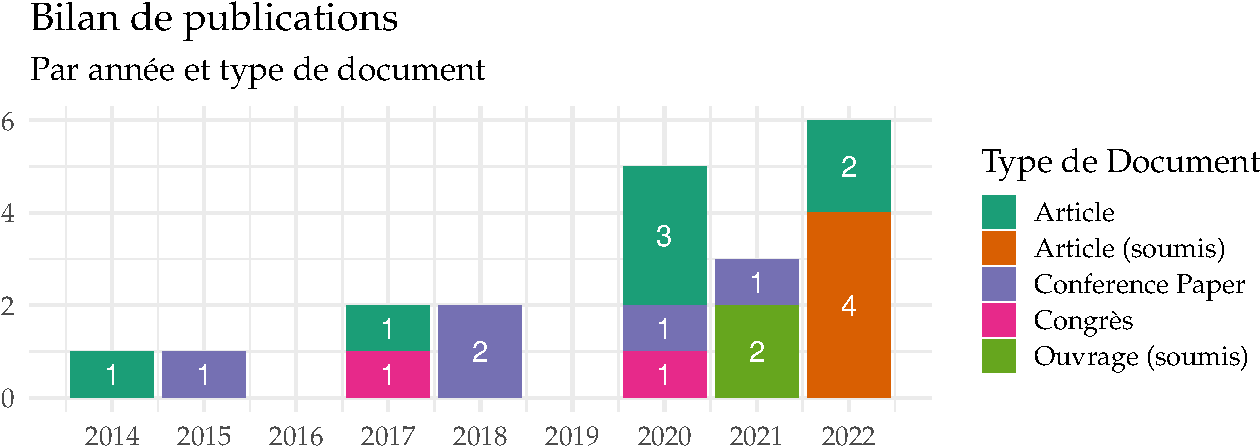
\includegraphics[width=0.95\textwidth,height=\textheight]{Figures/unnamed-chunk-3-1.pdf}

}

\end{figure}

Mes thématiques enseignement portent majoritairement sur XX

Je présente en détail le contenu pédagogique et de mes contributions aux
modules de formations qui donnent une aperçu de mes expériences
enseignement : (1) Recherche, Innovation et Développement, (2) Modules
de Licence AFTER, (3) Pôle Conception et Innovation Module Ingénierie de
l'innovation II / Design Thinking; et (4) Introduction au prototypage et
à l'impression 3D.

\hypertarget{participation-aux-modules-puxe9dagogiques}{%
\subsection{Participation aux modules
pédagogiques}\label{participation-aux-modules-puxe9dagogiques}}

\hypertarget{module-ci15recherche-innovation-et-duxe9veloppement}{%
\subsection{Module CI15--Recherche, Innovation et
Développement}\label{module-ci15recherche-innovation-et-duxe9veloppement}}

Ce module a pour objectif de faire une introduction à la méthode
scientifique afin de maîtriser les concepts et étapes clés d'un
processus de recherche. Le public visé sont des étudiants de 3ème année
ingénieur (BAC+ 5) et l'ensemble des étudiants de Master Design (BAC+ 5)
IDEAS (Innovation et Design Évalués par les Usages), Master Urbanisme et
Aménagement IUVTT (Innovation Urbaine pour des Villes \& Territoires en
Transformation) de l'ENSGSI.

Ce module permet d'acquérir les compétences suivantes :

\begin{itemize}
\tightlist
\item
  Avoir une compréhension sur les étapes de la méthode scientifique en
  identifiant le contexte, le problème de recherche, le cadre théorique,
  la méthodologies et les implications.
\item
  Avoir une connaissance globale sur les modes de financement de la
  recherche et l'importance sur la notion d'Open Science pour la France
  et l'EU.
\item
  Structurer une démarche de recherche documentaire ciblée
  (essentiellement en langue Anglaise) en identifiant des bases de
  données scientifiques pertinentes.
\item
  Savoir faire une analyse bibliométrique qualitative et quantitative à
  travers l'utilisation des outils de visualisation des réseaux et de
  gestion de références.
\item
  Développer une analyse critique des travaux de recherche, en utilisant
  une grille de lecture pour les articles scientifiques.
\item
  Planifier et mettre en œuvre un protocole expérimental de collecte des
  données en utilisant des méthodologies de recherche scientifique.
\item
  Synthétiser sous la forme de la rédaction d'un article la proposition
  d'un projet de recherche appliquée.
\end{itemize}

\textbf{Approche pédagogique:} Ce module est divisé en quatre séances
d'enseignement, avec deux grands volets: 1) méthodologie de la recherche
et 2) atelier d'écriture. Pour faire cela, les séquences pédagogiques
sont structurées sur une alternance entre cours magistraux et mises en
application de travaux dirigés au sein de séances. Chaque séance
comporte un travail à rendre à la fin de la séance.

Une spécificité de ce module concerne une attente pédagogique
particulière. Par le fait que les étudiants sont ad-portas à réaliser un
stage en entreprise pour valider le cycle d'ingénieur ou bien le diplôme
de Master M2, chaque étudiant doit faire une article d'état de l'art sur
l'objet de son stage hors des séances de cours en présentiel. Il s'agit
d'un premier écrit synthétique visant à mobiliser les outils vus en
cours pour analyser une thématique de leur choix en identifiant des
données / articles issues de la littérature scientifique pertinentes.
Cet écrit est révisé par un binôme d'enseignants, dont ils font un
retour afin d'améliorer et cadrer le problème et les attentes
scientifiques et industrielles. Un accompagnement tout au long de ce
processus de rédaction est proposé.

\textbf{Mes contributions à ce module :}

\begin{itemize}
\tightlist
\item
  Montage du module de formation en collaboration avec 1 enseignant de
  l'ENSGSI et 1 chercheur du laboratoire ERPI. D'abord pensé comme
  module de spécialisation, il est passé en 2020 dans le tronc commun
  des étudiants ingénieurs de dernière année et de Masters ENSGSI et
  IUVTT. Le nombre d'étudiants participant à la formation est donc passé
  d'une dizaine à une soixantaine.
\item
  Réalisation des séances cours magistral sur la méthodologie de
  recherche en identifiant des articles scientifiques support à la
  recherche en Innovation.
\item
  Animations de séances de travaux dirigés sur l'application de la
  méthode de revue systématique de la littérature à partir d'une
  équation ciblée.
\item
  Proposition d'un travail dirigé sur la recherche reproductible en
  utilisation de logiciels open source comme R et Github.
\item
  Développement de la plateforme Web support au cours avec pour le suivi
  et la publication des productions des étudiants:
  \url{https://ci15.netlify.app/}
\end{itemize}

\hypertarget{recyclage-des-matuxe9riaux-uxe0-laide-de-techniques-open-source-exploiter-durablement-les-ressources-et-les-partenariats}{%
\subsection{Recyclage des matériaux à l'aide de techniques open source /
Exploiter durablement les ressources et les
partenariats}\label{recyclage-des-matuxe9riaux-uxe0-laide-de-techniques-open-source-exploiter-durablement-les-ressources-et-les-partenariats}}

Les modules 1) Recyclage des matériaux à l'aide de techniques open
source, et 2), \emph{Exploiter durablement les ressources et les
partenariats} sont deux modules de la licence professionnelle
\emph{Animateur et facilitateur de tiers-lieux éco-responsables
(AFTER).} Cette licence est portée par l'ENSGSI et l'IUT Charlemagne à
Nancy et vise à former des personnes pouvant gérer et animer des tiers
lieux. Les tiers-lieux sont des nouveaux espaces socio-techniques qui se
font de plus en plus nombreux dans le cadre d'associations et des
organismes de l'Économie Sociale et Solidaire (ESS). Ils sont source de
médiation et d'innovation favorisant la co-creation, l'échange de
compétences sur des pratiques numériques et de fabrication pour les
citoyens, entrepreneurs, étudiants, salariés, artistes, etc qui veulent
expérimenter des nouvelles formes d'entreprenariat plus respectueux de
la planète. Le public visé (BAC+2) ont un profil intéressé par
l'approche de «faire soi-même» ayant une forte attention portée aux
enjeux environnementaux. :::

Ces deux modules permettent d'acquérir les compétences suivantes :

\begin{itemize}
\tightlist
\item
  Acquérir une culture et une philosophie de l'univers du « faire » :
  découvrir et comprendre les valeurs des tiers-lieux, fablabs
\item
  Identifier des initiatives et principales technologies utilisées pour
  la revalorisation de matériaux secondaires (plastique, bois) dans une
  approche de conception dites low tech et/out frugale.
\item
  Maîtriser le procédé de recyclage via injection plastique et
  utilisation de l'impression et
\item
  Création d'une animation autour de recyclage pour un publique ciblée.
\end{itemize}

\textbf{Approche pédagogique: }

Les deux modules sont basés sur une approche pédagogique par la
pratique. Le module de recyclage des matériaux à l'aide de techniques
open source est une introduction sur les étapes et les technologies
dites ``low tech'' dans le sens que sont appropriables et réplicables
par n'importe quel communaute tiers-lieux. Ce module valorise mes
travaux de recherche car les étudiants apprennent à identifier les types
de plastiques qui peuvent être réutilisables localement, à développer
une vision systémique sur la possible implantation de filières locales
afin de repérer les partenaires nécessaires à une future
démocratisation.

Concernant le module d'exploiter durablement les ressources et les
partenariats, le but est de sensibiliser les étudiants à la notion de
l'écologie industrielle, et surtout faire comprendre que les tiers lieux
peuvent être un levier pour mobiliser les acteurs de terrain en faveur
de la transition écologique. Cela s'inscrit dans la démarche « réduire,
réutiliser et recycler » de l'économie circulaire. Un case pédagogie
active est mise en place car les élèves doivent concevoir un atelier
pour un groupe d'élèves de l'enseignement secondaire avec un partenaire
éducatif local. Cette animation permet de découvrir les tiers lieux
comme des espaces d'expérimentation, de leur sensibiliser au recyclage
de matière plastique et enfin, de montrer le métier d' animateur tiers
lieux et de chercheur dans un même endroit.

Les étudiants découvrent des machines open source pour recyclage et
projets phares dans la communauté de recyclage et voir les objects que
peuvent être fabriques.

\textbf{Ma contribution:}

\begin{itemize}
\tightlist
\item
  Création des séquences pédagogiques pour les deux modules.
\item
  Développement et et supports techniques de l'open hardware
  (e.g.~machine d'injections manuel) utilisé pour l'animation d'un
  atelier d'introduction aux recyclage de matière plastiques avec la
  mise en application des outils technologiques présents au Green
  Fablab.
\item
  Création de supports pédagogiques aux enjeux sociétaux de l'économie
  circulaire axés sur le recyclage de matière plastique.
\item
  Montage et organisation de l'atelier pédagogique avec un public
  d'élèves de collège classé ``éducation prioritaire renforcé''
\end{itemize}

\hypertarget{introduction-uxe0-lage-du-faire-et-do-it-yourself-diy}{%
\subsection{Introduction à l'Age du faire et Do-It-Yourself
(DIY)}\label{introduction-uxe0-lage-du-faire-et-do-it-yourself-diy}}

Au cours de l'année 2022, J'ai eu l'opportunité de proposer un TP appelé
'\emph{Introduction à l'Age du faire et Do-It-Yourself (DIY)'} à
destination des étudiants de 2ème année cycle préparatoire ingénieur
(BAC+2) de l'ENSGSI. L'objectif est de les sensibiliser aux différentes
technologies qui permettent matérialiser et prototyper rapidement une
idée avec les technologies présentes dans le Lorraine Fab Living Lab et
le Green Fablab. Ce TP permet:

\begin{itemize}
\tightlist
\item
  Avoir une première connaissances sur les différentes technologies
  présentes dans le Lorraine Fab Living Lab mobilisés pour le
  prototypage et matérialisation physique et virtuel.
\item
  Formalization en utilisant un support collaborative
\end{itemize}

\textbf{Approche pédagogique: }

Cette démarche de « réduire, réutiliser et recycler » de l'économie
circulaire est applicable aussi dans le geste du prototypage et
maquettage dont les écoles d'ingénieurs font preuve. Avec l'expérience
des modules développés pour les étudiants de licence AFTER, deux séances
TP ont été implémentées courant décembre 2022 dans l'objectif de faire
une introduction sur la notion de matérialisation/prototypage physique
et matérialisation virtuelle.

La matérialisation physique eco-responsable est de montrer dans une
séance de 3h, voir une séquence pédagogique pour passer d'un esquisse
vers un prototype personnalisé recyclé. Les étudiants découvrent des
machines open source pour recyclage et projets phares dans la communauté
de recyclage et voir les objects que peuvent être fabriques.

Concernant la matérialisation virtuelle, l'objectif est de saisir les
possibilités que les environnement immersives et de réalité virtuel
permettent pour l'itération d'un concept. Donc, le pari est de
sensibiliser le plus tôt possible sur ces technologies afin que dans les
cursus du cycle ingénieur, les élèves ingénieurs puissent faire un
itération plus complète de conception de nouveau produit. Il a donc été
nécessaire d'en adapter le contenu et le format en fonction des
connaissances initiales des élèves car c'est une première opportunité de
prendre connaissance des méthodes de fabrication.

\textbf{Ma contribution: }

\begin{itemize}
\tightlist
\item
  Adaptation des outils de réalité virtuel développé dans le projet
  INEDIT pour l'usage pédagogique
\item
  Animations des séances pour l'introduction de design vectoriel et
  prototypage en 2D en lien avec les ressources technologiques du
  Lorraine Fab Living Lab.
\item
  Formalisation des étapes de prototypage en utilisant une plateforme
  pédagogique utilisé dans les cadres de Fablabs (e:g: FabManager)
\end{itemize}

Cette expérience a été très constructive d'un point de vue pédagogique
et ce travail pratique devrait être reconduit pour l'année 2023-2024.

\hypertarget{projet-denseignement}{%
\subsection{Projet d'enseignement}\label{projet-denseignement}}

Sur la base de l'expérience de création de cours pour les professeurs de
collèges et des lycées, et plus précisément les expériences de recherche
et la participation à des projets de recherche nationaux et européens,
mon projet pédagogique concerne donc l'application des génie de
conception mécanique en incluant des principes d'économie circulaire
afin que les future élèves ingénieurs identifient le contexte de
conception produit. Je peux le résumer en trois élément fondamentaux :

\begin{enumerate}
\def\labelenumi{\arabic{enumi}.}
\tightlist
\item
  La compréhension de la caractérisation des matériaux en utilisant
  l'approche open hardware comme support de fabrication afin de relever
  le comportement, et l'impact de fabrication traditionnels.
\item
  La conception de produit en utilisant des critères de soutenabilité
  tels que la réparabilité, le reconditionnement et le recyclage. Cette
  phase de conception peut inclure des aides technologiques à la
  créativité numérique comme la réalité virtuelle afin d'explorer un
  espace de conception plus large.
\item
  L'open source comme une pratique disruptive dans la conception
  mécanique et dans l'innovation produit.
\end{enumerate}

Mon constat de départ à travers des travaux de recherche préfigurent une
tendance forte dans la démocratisation des moyens de fabrication
numérique et dans la conception mécanique. L'un des enjeux majeurs
auxquels les futurs élèves ingénieurs vont faire face est de repenser
les moyens de production et les filières locales tout en gardant un axe
prioritaire sur la résilience des écosystèmes naturels. Ce paradoxe
n'est pas simple, et relève de compétences auxquels les espaces
d'innovation (éducatives, institutionnelles, publiques) comme les
fablabs peuvent donner des leviers d'action concrets.

D'abord, la compréhension et la caractérisation des matériaux est un
pilier essentiel dans la formation des ingénieurs. La communauté
scientifique développe de plus en plus de matériaux bio-sourcés. Il y a
un champ pédagogique à explorer en utilisant de nouveaux composites à
base de déchets qui impliquent la caractérisation des matériaux, ainsi
que des évaluations économiques et environnementales du cycle de vie.
Plus spécifiquement pour le cursus d'Ingénierie, il s'agit donc de créer
une connaissance de caractérisation mécanique open source pour
comprendre les impacts qu'ont les choix des procédés de fabrication sur
la performance mécanique. Assurément, un élément essentiel sera la
compréhension des barrières et des opportunités inhérentes à la matière
recyclée en tant que matière secondaire.

Ensuite, au vu des impacts écologiques de la surproduction et de
surconsommation sur la capacité de charge de nos écosystèmes, il est
impératif de favoriser des compétences pour prioriser le `droit à la
réparation' \footnote{Plus de détails dur la comunication officiel de
  l'EU:
  (https://www.europarl.europa.eu/news/en/headlines/society/20220331STO26410/why-is-the-eu-s-right-to-repair-legislation-important)}.
Le développement d'outils à faible coût, gratuits et à codes sources
ouverts, fabriqués numériquement (idéalement à partir de déchets
recyclés) pour permettre la création des moyens de production y compris
des outils scientifiques.

Et finalement, l'open source est très fédérateur dans la technologie de
l'information et des communications. Je peux imaginer que ce rôle
fédérateur l'open hardware peut aussi le faire grâce à la
démocratisation de l'électronique et de la fabrication numérique. Cela
pourra créer des nouvelles chaînes de valeur locales. L'approche
pédagogique doit mobiliser fortement les capacités à la création et à la
documentation en mode open source sur les concepts et prototypes dans
une communauté ouverte en dehors de la communauté académique.
Implémentées au sein des parcours ces compétences numériques nourrissent
la création pédagogique active que peut compléter les bases théoriques
autour de la conception mécanique et energétique.

Ce projet d'enseignement pourrait s'intituler \emph{``Conception de
produit soutenable open source : les atouts de la collecte jusqu'au
recyclage en circuit''} Ce parcours aurait pour objectif de combiner les
approches open hardware et \emph{Faire-soi-même} afin d'éco-concevoir
des produits et des procédés qui répondent aujourd'hui à la stratégie
des enjeux de l'économie circulaire.\\
L'objectif est de proposer un cheminement cohérent et progressif aux
étudiants en partant de l'analyse des besoins, co-créations de
solutions, et prototypage des objets de conception intermédiaire à
l'aide des techniques de l'impression 3D tout en identifiant une
réutilisation possible d'un gisement aujourd'hui non valorisable.

\hypertarget{activituxe9s-administratives-et-de-valorisation}{%
\section{Activités administratives et de
valorisation}\label{activituxe9s-administratives-et-de-valorisation}}

\hypertarget{activituxe9s-dencadrements-puxe9dagogique}{%
\subsection{Activités d'encadrements
pédagogique}\label{activituxe9s-dencadrements-puxe9dagogique}}

\begin{itemize}
\item
  2017-2018 Project Holipresse 1AI: Création d'un moule par système de
  strato-conception low-cost pour la fabrication de pièces injectées à
  partir de bouchons de bouteilles recyclés. Plus de détails:
  \url{https://holimaker.fr/}
\item
  Plast'If (2019- 2020): Test de caractérisation de matière plastique
  recyclée pour l'utilisation des machines d'impression directe -Fused
  Granular Fabrication FGF-. Plus de détails:
  \url{https://www.plastif.com/}
\item
  2017-2018: Project Fabcity Nancy 2AI: Cartographie des initiatives sur
  de démarches de fabrication locale et circulaire. Cette démarche est
  portée par ERPI / ARTEM / ENSAD. Plus de détails:
  \url{http://fabcity-nancy.fr/}
\item
  Accompagnement des étudiants (10) pendant 6 semaines dans le module
  d'Initiation de Recherche de l'école d'ingénieurs CESI Nancy. Création
  de prototypes pour l'extrusion de filaments en utilisant open
  hardware. Plus de détails dans le lien:
  \url{http://lf2l.fr/projects/green-fablab/}
\end{itemize}

\hypertarget{participation-coordination-et-montage-de-projets}{%
\subsection{Participation coordination et montage de
projets}\label{participation-coordination-et-montage-de-projets}}

\begingroup\fontsize{10}{12}\selectfont

\begin{tabu} to \linewidth {>{\raggedright\arraybackslash}p{1cm}>{\raggedright\arraybackslash}p{3cm}>{\raggedright\arraybackslash}p{2cm}>{\raggedright\arraybackslash}p{2cm}>{\raggedright}X}
\toprule
Projet & Financeur & Budget & Details & Role\\
\midrule
\addlinespace[0.3em]
\multicolumn{5}{l}{\textbf{2023 - ... }}\\
\hspace{1em}\cellcolor{gray!6}{Network to build and strengthen capacities in Climate Action through joint cocurricular programs, knowledge sharing and cooperation (LATAM-EU-CAN)} & \cellcolor{gray!6}{NA} & \cellcolor{gray!6}{NA} & \cellcolor{gray!6}{NA} & \cellcolor{gray!6}{NA}\\
\hspace{1em}Creating Innovation and entrepreneurship ecosystems (U4BUSINESS) & ERASMUS-LS & 900 k€ (dont 72 k€ pour ERPI) & NA & NA\\
\midrule
\hspace{1em}\cellcolor{gray!6}{Transnational Academy of Social Innovation for Climate Action} & \cellcolor{gray!6}{Erasmus+ KA220-HED - Cooperation partnerships in higher education.} & \cellcolor{gray!6}{Soumis Fev 2023} & \cellcolor{gray!6}{Le projet répond à la priorité de l'enseignement supérieur "Promouvoir des systèmes d'enseignement supérieur interconnectés" grâce à la structure de l'Académie, un réseau transnational de parties prenantes favorisant l'échange de compétences, d'expériences et de connaissances} & \cellcolor{gray!6}{Participation au montage et à la coordination de du ERPI}\\
\midrule
\hspace{1em}Everest Bio & NA & 60 k€ & Développer une méthodologie générique permettant d’évaluer les services écosystémiques rendus par des activités industrielles fonctionnant en circuit court afin d’améliorer la prise de décisions des acteurs industriels et du secteur public. Validation sur le cas d’une filière de recyclage du plastique en circuit court. & Participation au montage et à la coordination:\\
\midrule
\hspace{1em}\cellcolor{gray!6}{INEDIT (Open Innovation Ecosystems for Do It Together process)} & \cellcolor{gray!6}{EU Horizon 2020} & \cellcolor{gray!6}{6,4 M€} & \cellcolor{gray!6}{INEDIT entend contribuer, à travers la mobilisation d’une double plate-forme - numérique et physique – à renforcer le potentiel d’innovation des PMEs autour de la fabrication sociale.} & \cellcolor{gray!6}{Participation au montage et à la coordination du  task 6.4}\\
\hspace{1em}ClimateLabs & NA & 14 k€ & Renforcement des capacités de recherche appliquée et d'innovation de dix universités partenaires du Mexique, du Brésil et de la Colombie par la conception et la mise en œuvre de laboratoires d'innovation sociale pour l'atténuation et l'adaptation au changement climatique. & Participation au montage et à la coordination de Task 1.1 et Task 2.2\\
\hspace{1em}\cellcolor{gray!6}{Plast’if} & \cellcolor{gray!6}{Contrat Industriel} & \cellcolor{gray!6}{11 k€} & \cellcolor{gray!6}{Développement d'une méthodlogie pour permettre la discrimination des plastiques usagés destinés à être revalorisés par impression 3D granulés} & \cellcolor{gray!6}{Participation au montage et execution des taches tecjniques}\\
Green Compo 3D & ICEEL Intra-CARNOT & 14 000 €. & Valorisation en circuit court de déchets thermoplas-tiques pour la conception par impression 3D de structures composite & Execution du projet\\
\cellcolor{gray!6}{CPER SuschemProc (Chimie et Procédés Durables au service des industries lorraines)} & \cellcolor{gray!6}{ICEEL Intra-CARNOT} & \cellcolor{gray!6}{44 000 €.} & \cellcolor{gray!6}{Recyclage en circuit cout de différents matériaux plastiques de manière distribué et ce au moyen de machine d’impression 3D open source de type FDM (depôt de filament).} & \cellcolor{gray!6}{Execution du projet}\\
\bottomrule
\end{tabu}
\endgroup{}

\hypertarget{relations-avec-le-monde-publique}{%
\subsection{Relations avec le monde
publique}\label{relations-avec-le-monde-publique}}

\begin{itemize}
\item
  Module a été dispensé pour des étudiants et des industriels de la
  région de Costa Rica. La thématique a concerné l'identification des
  étapes dans un processus de création des projets d'innovation,
  l'évaluation prospective du degre de nouveauté en utilisation des
  technologies eye-tracking et neuro-lab (e.g.~capteurs physiologiques)
\item
  \textbf{2018:} Participation à l'organisation des congrès mondial des
  Fablabs --FAB14-- distribué en france. Un format distribué a été mis
  en place donc l'axe éducation à été organisé à Bataville, dans le
  Grand Est. Plus de détails dans le lien:
  \url{https://www.tierslieuxedu.org/2018-fab14edu-compte-rendu.pdf}
\item
  \textbf{2018-2019}: La ville de Nancy a développé un Conseil
  d'Orientation de la Transition Écologique de Nancy (COTEN) afin de
  mettre en place des objectifs et des actions pour trouver des
  solutions aux enjeux environnementaux. J'ai participé en tant que
  représentant du laboratoire ERPI entre 2018-2019 au groupe de travail
  sur la gestion des déchets.
\item
  \textbf{2017-2019}: Participation annuelle à la Foire Internationale
  de Nancy avec le stand de l'Université de Lorraine : Open Citizen Lab.
\end{itemize}

Plus précisément, un travail de médiation scientifique à la Foire
Internationale de Nancy pour les projets étudiants du LF2L. Dans ce
cadre, les prototypes des étudiants sont présentés pour avoir des
retours des utilisateurs. Cela est une activité pédagogique de
confrontation sur les idées développées hors du cadre conventionnel
académique. Egalement, mettre en place un stand du projet Green Fablab
afin de interagir avec les visiteur et vulgariser la
recherche.\footnote{\url{https://www.youtube.com/watch?v=c8ZyTJ9-YxU&feature=emb_title}}

\begin{itemize}
\tightlist
\item
  \textbf{2016} Participation au concours de vulgarisation scientifique
  \href{http://videos.univ-lorraine.fr/index.php?act=view&id=3475}{\textbf{Ma thèse en 180s (2016)}}\\
  Finale régionale : Ce concours permet aux doctorants de présenter leur
  sujet de recherche, en français et en termes simples, à un auditoire
  profane et diversifié. Chaque étudiant ou étudiante doit faire, en
  trois minutes, un exposé clair, concis et néanmoins convaincant sur
  son projet de recherche. J'ai pu participer lors de la finale
  Régionale, qui est le résultat d'un processus de sélection de 11
  doctorants sur une trentaine de candidats. J'ai obtenu le
  \textit{Prix des étudiants}, le prix du \textit{public} et la
  \(3^{ème}\) place après délibération du Jury.
\end{itemize}

Lien vers la vidéo de la prestation - Finale de l'Université de Lorraine
2016 : \url{https://videos.univ-lorraine.fr/index.php?act=view&id=3475}

\newpage

\hypertarget{bibliographie}{%
\section{Bibliographie}\label{bibliographie}}

\hypertarget{refs}{}
\begin{CSLReferences}{1}{0}
\leavevmode\vadjust pre{\hypertarget{ref-Bakshi2019b}{}}%
Bakshi, B.R., Ghosh, T., Lee, K., 2019. {Engineering, markets, and human
behavior: an essential integration for decisions toward sustainability}.
\url{https://doi.org/10.1016/j.coche.2019.10.004}

\leavevmode\vadjust pre{\hypertarget{ref-Barbier2019}{}}%
Barbier, E.B., 2019.
\href{https://academic.oup.com/oxrep/article/35/1/14/5267896}{{The
concept of natural capital}}. Oxford Rev. Econ. Policy 35, 14--36.

\leavevmode\vadjust pre{\hypertarget{ref-Ceschin2016}{}}%
Ceschin, F., Gaziulusoy, I., 2016. {Evolution of design for
sustainability: From product design to design for system innovations and
transitions}. Des. Stud. 47, 118--163.
\url{https://doi.org/10.1016/j.destud.2016.09.002}

\leavevmode\vadjust pre{\hypertarget{ref-Culot2020}{}}%
Culot, G., Nassimbeni, G., Orzes, G., Sartor, M., Nassimbeni, G., 2020.
{The future of manufacturing: a Delphi-based scenario analysis on
Industry 4.0}. Technol. Forecast. Soc. Change 120092.
https://doi.org/\url{https://doi.org/10.1016/j.techfore.2020.120092}

\leavevmode\vadjust pre{\hypertarget{ref-Despeisse2016}{}}%
Despeisse, M., Baumers, M., Brown, P., Charnley, F., Ford, S.J.,
Garmulewicz, A., Knowles, S., Minshall, T.H.W., Mortara, L.,
Reed-Tsochas, F.P., Rowley, J., 2017. {Unlocking value for a circular
economy through 3D printing: A research agenda}. Technol. Forecast. Soc.
Change 115, 75--84. \url{https://doi.org/10.1016/j.techfore.2016.09.021}

\leavevmode\vadjust pre{\hypertarget{ref-Dietz2006}{}}%
Dietz, S., Neumayer, E., 2007. {Weak and strong sustainability in the
SEEA: Concepts and measurement}. Ecol. Econ. 61, 617--626.
\url{https://doi.org/10.1016/j.ecolecon.2006.09.007}

\leavevmode\vadjust pre{\hypertarget{ref-Heikkinen2020a}{}}%
Heikkinen, I.T.S., Savin, H., Partanen, J., Seppälä, J., Pearce, J.M.,
2020. {Towards national policy for open source hardware research: The
case of Finland}. Technol. Forecast. Soc. Change 155, 119986.
\url{https://doi.org/10.1016/j.techfore.2020.119986}

\leavevmode\vadjust pre{\hypertarget{ref-Herrmann2020}{}}%
Herrmann, C., Juraschek, M., Burggräf, P., Kara, S., 2020. {Urban
production: State of the art and future trends for urban factories}.
CIRP Ann. 69, 764--787. \url{https://doi.org/10.1016/j.cirp.2020.05.003}

\leavevmode\vadjust pre{\hypertarget{ref-IPBS2019}{}}%
IPBS, 2019.
\href{https://ipbes.net/global-assessment\%7B/\%\%7D0Ahttps://ipbes.net/global-assessment-report-biodiversity-ecosystem-services}{{Global
assessment report on biodiversity and ecosystem services of the
Intergovernmental Science-Policy Platform on Biodiversity and Ecosystem
Services}}.

\leavevmode\vadjust pre{\hypertarget{ref-IPCC2017}{}}%
IPCC, 2017.
\href{https://www.ipcc.ch/report/sixth-assessment-report-working-group-i/}{{AR6
Climate Change 2021: The Physical Science Basis --- IPCC}}.

\leavevmode\vadjust pre{\hypertarget{ref-Jacobi2022}{}}%
Jacobi, J., Llanque, A., Mukhovi, S.M., Birachi, E., Groote, P. von,
Eschen, R., Hilber-Schöb, I., Kiba, D.I., Frossard, E., Robledo-Abad,
C., 2022. {Transdisciplinary co-creation increases the utilization of
knowledge from sustainable development research}. Environ. Sci. Policy
129, 107--115. \url{https://doi.org/10.1016/j.envsci.2021.12.017}

\leavevmode\vadjust pre{\hypertarget{ref-Kleer2019}{}}%
Kleer, R., Piller, F.T., 2019. {Local manufacturing and structural
shifts in competition: Market dynamics of additive manufacturing}. Int.
J. Prod. Econ. 216, 23--34.
\url{https://doi.org/10.1016/j.ijpe.2019.04.019}

\leavevmode\vadjust pre{\hypertarget{ref-Liu2019g}{}}%
Liu, X., Bakshi, B.R., 2019. {Ecosystem Services in Life Cycle
Assessment while Encouraging Techno‐Ecological Synergies}. J. Ind. Ecol.
23, 347--360. \url{https://doi.org/10.1111/jiec.12755}

\leavevmode\vadjust pre{\hypertarget{ref-Pearce2020a}{}}%
Pearce, J.M., 2020. {Economic savings for scientific free and open
source technology: A review}. HardwareX 8, e00139.
\url{https://doi.org/10.1016/j.ohx.2020.e00139}

\leavevmode\vadjust pre{\hypertarget{ref-Pearce2017b}{}}%
Pearce, J.M., 2017. {Impacts of open source hardware in science and
engineering}. Bridge 47, 24--31.

\leavevmode\vadjust pre{\hypertarget{ref-Wu2021a}{}}%
Wu, H., Mehrabi, H., Karagiannidis, P., Naveed, N., 2022. {Additive
manufacturing of recycled plastics: Strategies towards a more
sustainable future}. J. Clean. Prod. 335, 130236.
\url{https://doi.org/10.1016/j.jclepro.2021.130236}

\end{CSLReferences}

\appendix

\hypertarget{annexes}{%
\section*{Annexes}\label{annexes}}
\addcontentsline{toc}{section}{Annexes}

\hypertarget{articles}{%
\subsection{Liste de la Production Scientifique}\label{articles}}

\hypertarget{articles-uxe0-comituxe9-de-lecture-dans-des-revues-internationales}{%
\subsubsection{Articles à comité de lecture dans des revues
internationales}\label{articles-uxe0-comituxe9-de-lecture-dans-des-revues-internationales}}

\begin{enumerate}
\def\labelenumi{\arabic{enumi}.}
\item
  Gabriel, A., \textbf{Cruz, F.}, 2023. Open source IoT-based collection
  bin applied to local plastic recycling. HardwareX 13, e00389.
  \url{https://doi.org/10.1016/j.ohx.2022.e00389}
\item
  López, V.M., Carou, D., \textbf{Cruz S, F.A.}, 2022. Feasibility study
  on the use of recycled materials for prototyping purposes: A
  comparative study based on the tensile strength. Proceedings of the
  Institution of Mechanical Engineers, Part B: Journal of Engineering
  Manufacture 09544054221113378.
  \url{https://doi.org/10.1177/09544054221113378}
\item
  Xue, F., Robin, G., Boudaoud, H., \textbf{Cruz Sanchez, F.A.}, Daya,
  E.M., 2022. General Methodology to Investigate the Effect of Process
  Parameters on the Vibration Properties of Structures Produced by
  Additive Manufacturing Using Fused Filament Fabrication. JOM 74,
  1166--1175. \url{https://doi.org/10.1007/s11837-021-05051-9}
\item
  Santander, P., \textbf{Cruz Sanchez, F.A}., Boudaoud, H., Camargo, M.,
  2022. Social, political, and technological dimensions of the
  sustainability evaluation of a recycling network. A literature review.
  Clean. Eng. Technol. \url{https://doi.org/10.1016/j.clet.2022.100397}
\item
  Alexandre, A., \textbf{Cruz Sanchez, F.A.}, Boudaoud, H., Camargo, M.,
  Pearce, J.M., 2020. Mechanical Properties of Direct Waste Printing of
  Polylactic Acid with Universal Pellets Extruder: Comparison to Fused
  Filament Fabrication on Open-Source Desktop Three-Dimensional
  Printers. 3D Print. Addit. Manuf. 3dp.2019.0195.
  \url{https://doi.org/10.1089/3dp.2019.0195}
\item
  Santander, P., \textbf{Cruz Sanchez, F.A.}, Boudaoud, H., Camargo, M.,
  2020. Closed loop supply chain network for local and distributed
  plastic recycling for 3D printing: a MILP-based optimization approach.
  Resour. Conserv. Recycl. 154, 104531.
  \url{https://doi.org/10.1016/j.resconrec.2019.104531}
\item
  \textbf{Cruz Sanchez, F.A.}, Boudaoud, H., Camargo, M., Pearce, J.M.,
  2020. Plastic recycling in additive manufacturing: A systematic
  literature review and opportunities for the circular economy. J.
  Clean. Prod. 264, 121602.
  \url{https://doi.org/10.1016/j.jclepro.2020.121602}
\item
  \textbf{Cruz Sanchez, F.A.}, Boudaoud, H., Hoppe, S., Camargo, M.,
  2017. Polymer recycling in an open-source additive manufacturing
  context: Mechanical issues. Addit. Manuf. 17, 87--105.
  \url{https://doi.org/10.1016/j.addma.2017.05.013}
\item
  \textbf{Cruz Sanchez, F.A.}, Boudaoud, H., Muller, L., Camargo, M.,
  2014. Towards a standard experimental protocol for open source
  additive manufacturing. Virtual Phys. Prototyp. 9, 151--167.
  https://doi.org/10.1080/17452759.2014.919553
\end{enumerate}

\hypertarget{articles-soumis-ruxe9cemment-en-attente-de-duxe9cision}{%
\subsubsection{Articles soumis récemment (en attente de décision)
:}\label{articles-soumis-ruxe9cemment-en-attente-de-duxe9cision}}

\begin{enumerate}
\def\labelenumi{\arabic{enumi}.}
\tightlist
\item
  Xue, F., Robin, G., Boudaoud, H., \textbf{Cruz Sanchez, F.A.}, Daya,
  E.M.,\emph{``Enhancing vibration damping properties of viscoelastic
  structures printed by fused filament fabrication through the
  optimization of process parameters''}. Journal of Manufacturing
  Processes.\textbf{(Soumis en Mars 2023-- en révision)}
\end{enumerate}

\begin{enumerate}
\def\labelenumi{\arabic{enumi}.}
\item
  Osorio F, \textbf{Cruz Sanchez F}, Camargo M., Dupont L.,Peña J.,
  \emph{``Exploring team roles for social innovation labs: toward a
  competence-based role self-assessment approach''} Journal of
  Engineering and Technology Management \textbf{(Soumis en Mars 2022--
  en révision)}
\item
  Osorio F, \textbf{Cruz Sanchez F}, Camargo M., Dupont L.,Peña J.,
  \emph{``Exploring team roles for social innovation labs: toward a
  competence-based role self-assessment approach''} Journal of
  Engineering and Technology Management \textbf{(Soumis en Mars 2022--
  en révision)}
\end{enumerate}

\hypertarget{communications-dans-des-congruxe8s-internationaux-uxe0-comituxe9-de-lecture}{%
\subsubsection{Communications dans des congrès internationaux à comité
de
lecture}\label{communications-dans-des-congruxe8s-internationaux-uxe0-comituxe9-de-lecture}}

\begin{enumerate}
\def\labelenumi{\arabic{enumi}.}
\item
  Xue, F., Robin, G., Boudaoud, H., \textbf{Cruz Sanchez, F. A.}, \&
  Daya, E. M. (2021). Effect of process parameters on the vibration
  properties of PLA structure fabricated by additive manufacturing. In
  2021 International Solid Freeform Fabrication Symposium. University of
  Texas at Austin.
\item
  Roux-Marchand, T., \textbf{Cruz, F}., Dupont, L., Camargo, M., Osorio,
  F., 2020. Connecting the strategic intent of innovation labs and
  projects: the case of the Green Fablab, in: 2020 IEEE International
  Conference on Engineering, Technology and Innovation (ICE/ITMC). IEEE,
  pp.~1--10. https://doi.org/10.1109/ICE/ITMC49519.2020.9198320
\item
  Pavlo, S., \textbf{Fabio, C}., Hakim, B., Mauricio, C., 2018.
  3D-Printing Based Distributed Plastic Recycling: A Conceptual Model
  for Closed-Loop Supply Chain Design, in: 2018 IEEE International
  Conference on Engineering, Technology and Innovation (ICE/ITMC). IEEE,
  pp.~1--8. https://doi.org/10.1109/ICE.2018.8436296
\item
  Albuquerque, R., Arbelaez, G., \textbf{Cruz, F.}, Camargo, M., Joseph,
  D., Tran, N., 2018. Modelling, Printing and Validation of Dental Dry
  Models for Implantology Skills Training, in: 2018 IEEE International
  Conference on Engineering, Technology and Innovation (ICE/ITMC). IEEE,
  pp.~1--8. https://doi.org/10.1109/ICE.2018.8436302
\item
  \textbf{Cruz, F.}, Lanza, S., Boudaoud, H., Hoppe, S., Camargo, M.,
  2015. Polymer Recycling and Additive Manufacturing in an Open Source
  context : Optimization of processes and methods, in: Solid Freeform
  Fabrication. Austin, Texas, pp.~1591--1600.
\end{enumerate}

\hypertarget{ouvrages-scientifiques}{%
\subsubsection{Ouvrages scientifiques}\label{ouvrages-scientifiques}}

\begin{enumerate}
\def\labelenumi{\arabic{enumi}.}
\item
  \textbf{Cruz, F.}, Lanza, S., Boudaoud, H., Hoppe, S., Camargo, M.,
  \emph{``Approche méthodologique pour évaluer la faisabilité du
  recyclage des polymères dans un contexte de fabrication additive
  open-source.''} (En relecture par les éditeurs)
\item
  Pavlo, S., \textbf{Fabio, C.}, Hakim, B., Mauricio,
  C.,\emph{``Recyclage distribué en circuit court de plastiques
  revalorisés par l'impression 3D « Open Source »: Un cadre pour
  l'analyse et l'évaluation de sa durabilité''.} (En relecture par les
  éditeurs)
\end{enumerate}

\hypertarget{colloques-et-congruxe8s-nationales}{%
\subsubsection{Colloques et congrès
nationales}\label{colloques-et-congruxe8s-nationales}}

\begin{enumerate}
\def\labelenumi{\arabic{enumi}.}
\item
  Marche, B., Kasmi, F., \textbf{Sanchez, F.}, Mayer, F., \& Dupont, L.
  (2020, March). From technological demonstrator to sustainable supply
  chain demonstrator: a conceptual framework. In Spring of Innovation.
\item
  \textbf{Fabio Cruz}, Hakim Boudaoud, Sandrine Hoppe, Mauricio Camargo.
  Le concept du Green Fablab: une approche distribuée pour le recyclage
  de polymères en circuit-court dans le cadre de la fabrication additive
  open-source. 15ème Congrès de la Société Française de Génie des
  Procédés (SFGP), Jul 2017, Nancy, France. ⟨hal-02518997⟩
\end{enumerate}

\newpage

\hypertarget{les-attestations-de-lensemble-des-enseignements-dispensuxe9s}{%
\subsection{Les attestations de l'ensemble des enseignements
dispensés}\label{les-attestations-de-lensemble-des-enseignements-dispensuxe9s}}

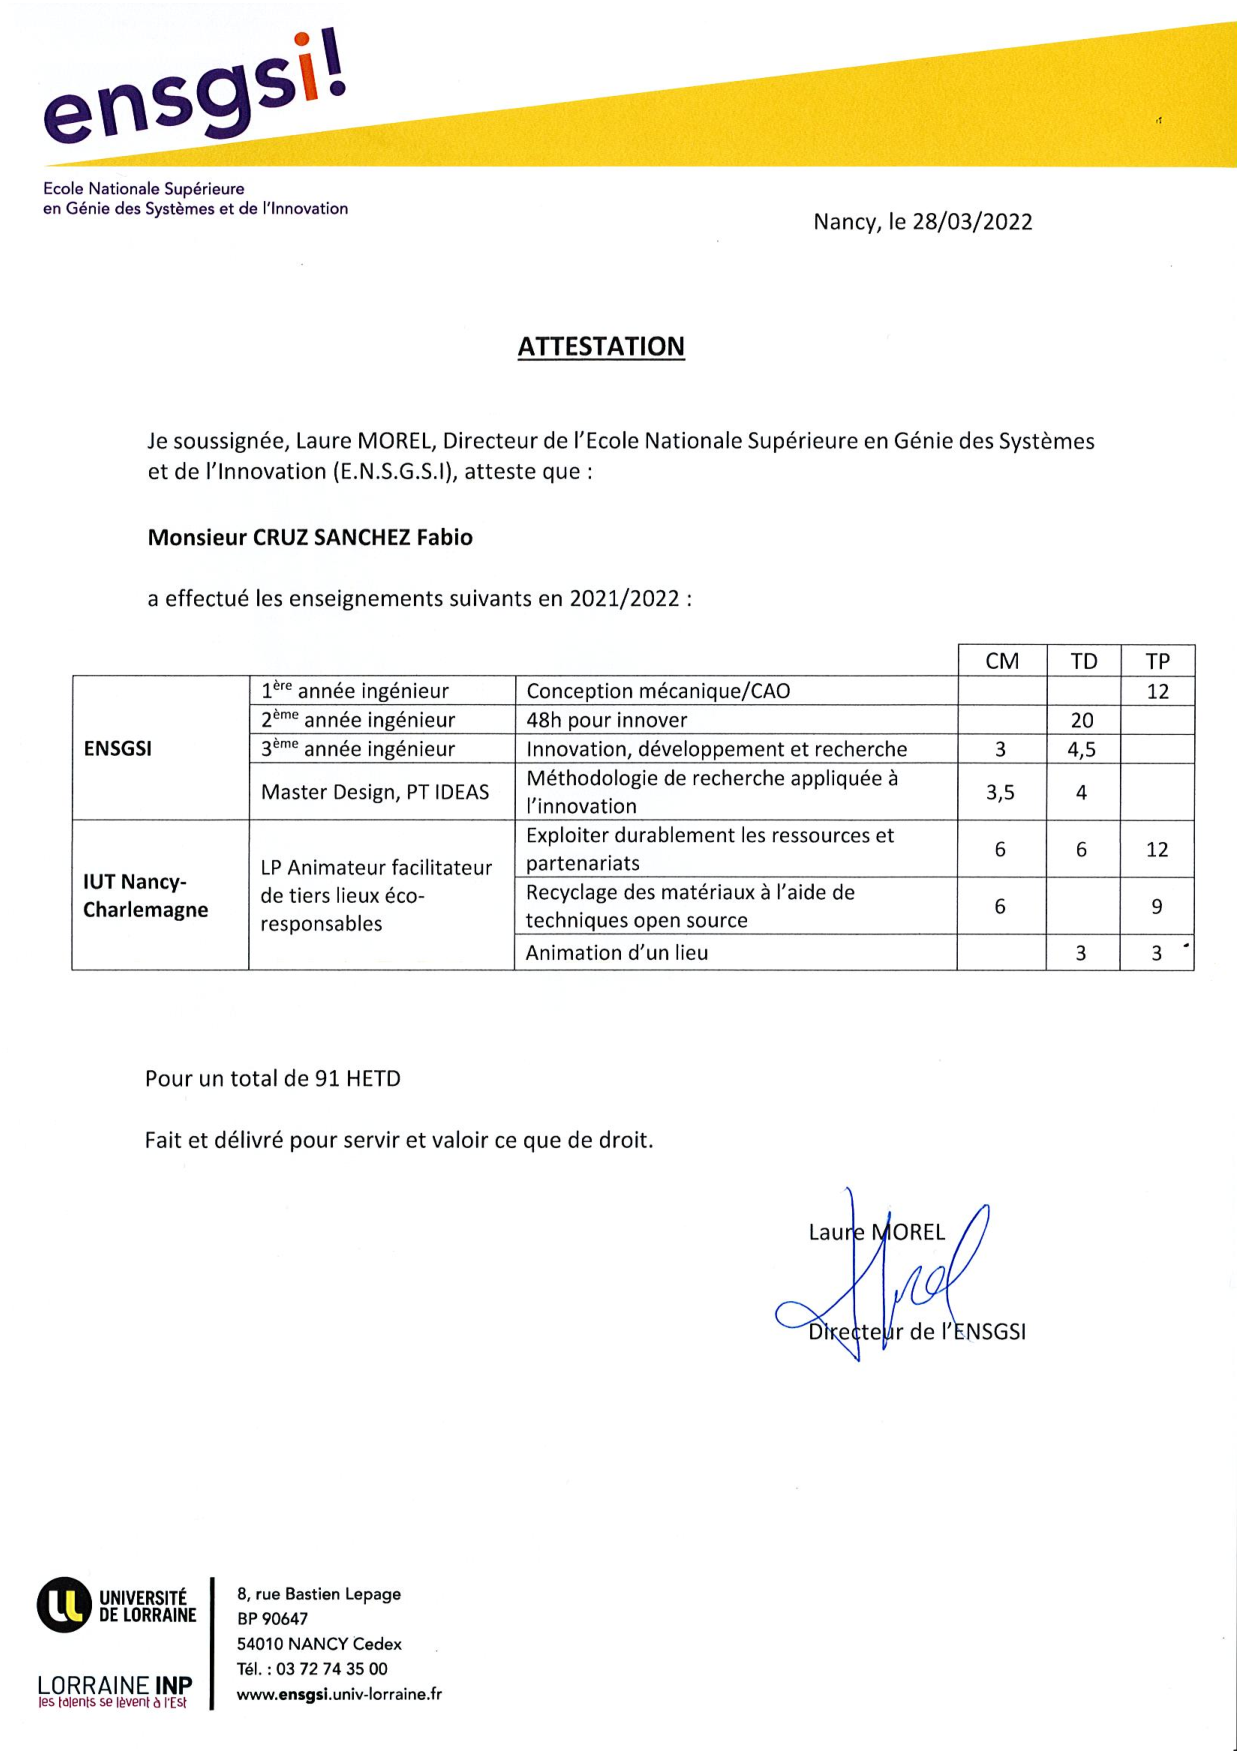
\includepdf[pages=-]{./annexs/Heures.pdf}



\end{document}
